% appendix/rcuimpl/rcutreewt.tex

\section{Hierarchical RCU Code Walkthrough}
\label{app:rcuimpl:rcutreewt:Hierarchical RCU Code Walkthrough}

This section walks through selected sections of the Linux-kernel
hierarchical RCU code.
As such, this section is intended for hard-core hackers who wish
to understand hierarchical RCU at a very low level, and such hackers
should first read
Section~\ref{app:rcuimpl:rcutree:Hierarchical RCU Overview}.
Hard-core masochists might also be interested in reading this section.
Of course \emph{really} hard-core masochists will read this section
before reading
Section~\ref{app:rcuimpl:rcutree:Hierarchical RCU Overview}.

Section~\ref{app:rcuimpl:rcutreewt:Data Structures and Kernel Parameters}
describes data structures and kernel parameters,
Section~\ref{app:rcuimpl:rcutreewt:External Interfaces}
covers external function interfaces,
Section~\ref{app:rcuimpl:rcutreewt:Initialization}
presents the initialization process,
Section~\ref{app:rcuimpl:rcutreewt:CPU Hotplug}
explains the CPU-hotplug interface,
Section~\ref{app:rcuimpl:rcutreewt:Miscellaneous Functions}
covers miscellaneous utility functions,
Section~\ref{app:rcuimpl:rcutreewt:Grace-Period-Detection Functions}
describes the mechanics of grace-period detection,
Section~\ref{app:rcuimpl:rcutreewt:Dyntick-Idle Functions}
presents the dynticks-idle interface,
Section~\ref{app:rcuimpl:rcutreewt:Forcing Quiescent States}
covers the functions that handle holdout CPUs (including offline and
dynticks-idle CPUs), and
Section~\ref{app:rcuimpl:rcutreewt:CPU-Stall Detection}
presents functions that report on stalled CPUs, namely those spinning
in kernel mode for many seconds.
Finally,
Section~\ref{app:rcuimpl:rcutreewt:Possible Flaws and Changes}
reports on possible design flaws and fixes.

\subsection{Data Structures and Kernel Parameters}
\label{app:rcuimpl:rcutreewt:Data Structures and Kernel Parameters}

A full understanding of the Hierarchical RCU data structures is
critically important to understanding the algorithms.
To this end,
Section~\ref{app:rcuimpl:rcutreewt:Tracking Dyntick State}
describes the data structures used to track each CPU's dyntick-idle state,
Section~\ref{app:rcuimpl:rcutreewt:Nodes in the Hierarchy}
describes the fields in the per-node data structure making up the
\co{rcu_node} hierarchy,
Section~\ref{app:rcuimpl:rcutreewt:Per-CPU Data}
describes per-CPU \co{rcu_data} structure,
Section~\ref{app:rcuimpl:rcutreewt:RCU Global State}
describes the field in the global \co{rcu_state} structure,
and
Section~\ref{app:rcuimpl:rcutreewt:Kernel Parameters}
describes the kernel parameters that control Hierarchical RCU's
operation.

Figure~\ref{fig:app:rcuimpl:rcutree:Hierarchical RCU State With Dynticks}
on
Page~\pageref{fig:app:rcuimpl:rcutree:Hierarchical RCU State With Dynticks}
and
Figure~\ref{fig:app:rcuimpl:rcutree:Initialized RCU Data Layout}
on
Page~\pageref{fig:app:rcuimpl:rcutree:Initialized RCU Data Layout}
can be very helpful in keeping one's place through the following detailed
data-structure descriptions.

\subsubsection{Tracking Dyntick State}
\label{app:rcuimpl:rcutreewt:Tracking Dyntick State}

The per-CPU \co{rcu_dynticks} structure tracks dynticks state using the
following fields:

\begin{itemize}
\item	\co{dynticks_nesting}:
	This \co{int} counts the number of reasons that the corresponding
	CPU should be monitored for RCU read-side critical sections.
	If the CPU is in dynticks-idle mode, then this counts the
	irq nesting level, otherwise it is one greater than the
	irq nesting level.
\item	\co{dynticks}:
	This \co{int} counter's value is even if the corresponding CPU is
	in dynticks-idle mode and there are no irq handlers currently
	running on that CPU, otherwise the counter's value is odd.
	In other words, if this counter's value is odd, then the
	corresponding CPU might be in an RCU read-side critical section.
\item	\co{dynticks_nmi}:
	This \co{int} counter's value is odd if the corresponding CPU is
	in an NMI handler, but only if the NMI arrived while this
	CPU was in dyntick-idle mode with no irq handlers running.
	Otherwise, the counter's value will be even.
\end{itemize}

This state is shared between the rcu and rcu\_bh implementations.

\subsubsection{Nodes in the Hierarchy}
\label{app:rcuimpl:rcutreewt:Nodes in the Hierarchy}

As noted earlier, the \co{rcu_node} hierarchy is flattened into
the \co{rcu_state} structure as shown in
Figure~\ref{fig:app:rcuimpl:rcutree:Mapping rcu-node Hierarchy Into Array}
on
page~\pageref{fig:app:rcuimpl:rcutree:Mapping rcu-node Hierarchy Into Array}.
Each \co{rcu_node} in this hierarchy has fields as follows:

\begin{itemize}
\item	\co{lock}:
	This spinlock guards the non-constant fields in this structure.
	This lock is acquired from softirq context, so must disable
	irqs.

\QuickQuiz{}
	Why not simply disable bottom halves (softirq) when acquiring
	the \co{rcu_data} structure's \co{lock}?
	Wouldn't this be faster?
\QuickQuizAnswer{
	Because this lock can be acquired from functions
	called by \co{call_rcu()}, which in turn can be
	invoked from irq handlers.
	Therefore, irqs \emph{must} be disabled when
	holding this lock.
} \QuickQuizEnd

	The \co{lock} field of the root \co{rcu_node} has additional
	responsibilities:
	\begin{enumerate}
	\item	Serializes CPU-stall checking, so that a given stall
		is reported by only one CPU.
		This can be important on systems with thousands of
		CPUs!
	\item	Serializes starting a new grace period, so that
		multiple CPUs don't start conflicting grace periods
		concurrently.
	\item	Prevents new grace periods from starting in code that
		needs to run within the confines of a single grace period.
	\item	Serializes the state machine forcing quiescent states
		(in \co{force_quiescent_state()}) in order to
		keep the number of reschedule IPIs down to a dull
		roar.
	\end{enumerate}
\item	\co{qsmask}:
	This bitmask tracks which CPUs (for leaf \co{rcu_node} structures)
	or groups of CPUs (for non-leaf \co{rcu_node} structures)
	still need to pass through a quiescent state in order for the
	current grace period to end.
\item	\co{qsmaskinit}:
	This bitmask tracks which CPUs or groups of CPUs will need to
	pass through a quiescent state for subsequent grace periods
	to end.
	The online/offline code manipulates the \co{qsmaskinit} fields,
	which are copied to the corresponding \co{qsmask} fields at
	the beginning of each grace period.
	This copy operation is one reason why grace period initialization
	must exclude online/offline operations.
\item	\co{grpmask}:
	This bitmask has a single bit set, and that is the bit corresponding
	to the this \co{rcu_node} structure's position in the parent
	\co{rcu_node} structure's \co{qsmask} and \co{qsmaskinit}
	fields.
	Use of this field simplifies quiescent-state processing,
	as suggested by Manfred Spraul.

\QuickQuiz{}
	How about the \co{qsmask} and \co{qsmaskinit}
	fields for the leaf \co{rcu_node} structures?
	Doesn't there have to be some way to work out
	which of the bits in these fields corresponds
	to each CPU covered by the \co{rcu_node} structure
	in question?
\QuickQuizAnswer{
	Indeed there does!
	The \co{grpmask} field in each CPU's \co{rcu_data}
	structure does this job.
} \QuickQuizEnd

\item	\co{grplo}:
	This field contains the number of the lowest-numbered CPU covered
	by this \co{rcu_node} structure.
\item	\co{grphi}:
	This field contains the number of the highest-numbered CPU covered
	by this \co{rcu_node} structure.
\item	\co{grpnum}:
	This field contains the bit number in the parent \co{rcu_node}
	structure's \co{qsmask} and \co{qsmaskinit} fields that this
	\co{rcu_node} structure corresponds to.
	In other words, given a pointer \co{rnp} to a given
	\co{rcu_node} structure, it will always be the case that
	\co{1UL << rnp->grpnum == rnp->grpmask}.
	The \co{grpnum} field is used only for tracing output.
\item	\co{level}:
	This field contains zero for the root \co{rcu_node} structure,
	one for the \co{rcu_node} structures that are children of
	the root, and so on down the hierarchy.
\item	\co{parent}:
	This field is a pointer to the parent \co{rcu_node} structure,
	or NULL for the root \co{rcu_node} structure.
\end{itemize}

\subsubsection{Per-CPU Data}
\label{app:rcuimpl:rcutreewt:Per-CPU Data}

The \co{rcu_data} structure contains RCU's per-CPU state.
It contains control variables governing grace periods and
quiescent states (\co{completed}, \co{gpnum}, \co{passed_quiesc_completed},
\co{passed_quiesc}, \co{qs_pending}, \co{beenonline}, \co{mynode},
and \co{grpmask}).
The \co{rcu_data} structure also contains control variables pertaining
to RCU callbacks
(\co{nxtlist}, \co{nxttail}, \co{qlen}, and \co{blimit}).
Kernels with dynticks enabled will have relevant control variables in
the \co{rcu_data} structure
(\co{dynticks}, \co{dynticks_snap}, and \co{dynticks_nmi_snap}).
The \co{rcu_data} structure contains event counters used by tracing
(\co{dynticks_fqs} given dynticks, \co{offline_fqs}, and \co{resched_ipi}).
Finally, a pair of fields count calls to \co{rcu_pending()} in order
to determine when to force quiescent states (\co{n_rcu_pending} and
\co{n_rcu_pending_force_qs}), and a \co{cpu} field indicates which
CPU to which a given \co{rcu_data} structure corresponds.

Each of these fields is described below.

\begin{itemize}
\item	\co{completed}:
	This field contains the number of the most recent grace period
	that this CPU is aware of having completed.
\item	\co{gpnum}:
	This field contains the number of the most recent grace period
	that this CPU is aware of having started.
\item	\co{passed_quiesc_completed}:
	This field contains the number of the grace period that had most
	recently completed when this
	CPU last passed through a quiescent state.
	The ``most recently completed'' will be from the viewpoint of
	the CPU passing through the quiescent state: if the CPU is
	not yet aware that grace period (say) 42 has completed, it
	will still record the old value of 41.
	This is OK, because the only way that the grace period can
	complete is if this CPU has already passed through a
	quiescent state.
	This field is initialized to a (possibly mythical) past
	grace period number to avoid race conditions when booting
	and when onlining a CPU.
\item	\co{passed_quiesc}:
	This field indicates whether this CPU has passed
	through a quiescent state since the grace period number
	stored in \co{passed_quiesc_completed} completed.
	This field is cleared each time the corresponding CPU
	becomes aware of the start of a new grace period.
\item	\co{qs_pending}:
	This field indicates that this CPU is aware that the core
	RCU mechanism is waiting for it to pass through a quiescent state.
	This field is set to one when the CPU detects a new grace
	period or when a CPU is coming online.

\QuickQuiz{}
	But why bother setting \co{qs_pending} to one when a CPU
	is coming online, given that being offline is an extended
	quiescent state that should cover any ongoing grace period?
\QuickQuizAnswer{
	Because this helps to resolve a race between a CPU coming online
	just as a new grace period is starting.
} \QuickQuizEnd

\QuickQuiz{}
	Why record the last completed grace period number in
	\co{passed_quiesc_completed}?
	Doesn't that cause this RCU implementation to be vulnerable
	to quiescent states seen while no grace period was in progress
	being incorrectly applied to the next grace period that starts?
\QuickQuizAnswer{
	We record the last completed grace period number in order
	to avoid races where a quiescent state noted near the end of
	one grace period is incorrectly applied to the next grace
	period, especially for dyntick and CPU-offline grace periods.
	Therefore, \co{force_quiescent_state()} and friends all
	check the last completed grace period number to avoid such races.

	Now these dyntick and CPU-offline grace periods are only checked
	for when a grace period is actually active.
	The only quiescent states that can be recorded when no grace
	period is in progress are self-detected quiescent states,
	which are recorded in the \co{passed_quiesc_completed},
	\co{passed_quiesc}, and \co{qs_pending}.
	These variables are initialized every time the corresponding
	CPU notices that a new grace period has started, preventing
	any obsolete quiescent states from being applied to the
	new grace period.

	All that said, optimizing grace-period latency may require that
	\co{gpnum} be tracked in addition to \co{completed}.
} \QuickQuizEnd

\item	\co{beenonline}:
	This field, initially zero, is set to one whenever the corresponding
	CPU comes online.
	This is used to avoid producing useless tracing output for CPUs
	that never have been online, which is useful in kernels where
	\co{NR_CPUS} greatly exceeds the actual number of CPUs.

\QuickQuiz{}
	What is the point of running a system with \co{NR_CPUS}
	way bigger than the actual number of CPUs?
\QuickQuizAnswer{
	Because this allows producing a single binary of the Linux kernel
	that runs on a wide variety of systems, greatly easing administration
	and validation.
} \QuickQuizEnd

\item	\co{mynode}:
	This field is a pointer to the leaf \co{rcu_node} structure that
	handles the corresponding CPU.
\item	\co{grpmask}:
	This field is a bitmask that has the single bit set that indicates
	which bit in \co{mynode->qsmask} signifies the corresponding CPU.
\item	\co{nxtlist}:
	This field is a pointer to the oldest RCU callback (\co{rcu_head}
	structure) residing on this CPU, or \co{NULL} if this CPU currently
	has no such callbacks.
	Additional callbacks may be chained via their \co{next} pointers.
\item	\co{nxttail}:
	This field is an array of double-indirect tail pointers
	into the \co{nxtlist} callback list.
	If \co{nxtlist} is empty, then all of the \co{nxttail} pointers
	directly reference the \co{nxtlist} field.
	Each element of the \co{nxttail} array has meaning as follows:
	\begin{itemize}
	\item	\co{RCU_DONE_TAIL=0}:
		This element references the \co{->next} field of
		the last callback that has passed through its grace
		period and is ready to invoke, or references the \co{nxtlist}
		field if there is no such callback.
	\item	\co{RCU_WAIT_TAIL=1}:
		This element references the \co{next} field of the
		last callback that is waiting for the current grace
		period to end, or is equal to the \co{RCU_DONE_TAIL}
		element if there is no such callback.
	\item	\co{RCU_NEXT_READY_TAIL=2}:
		This element references the \co{next} field of the
		last callback that is ready to wait for the next
		grace period, or is equal to the \co{RCU_WAIT_TAIL}
		element if there is no such callback.
	\item	\co{RCU_NEXT_TAIL=3}:
		This element references the \co{next} field of the
		last callback in the list, or references the \co{nxtlist}
		field if the list is empty.
	\end{itemize}

\QuickQuiz{}
	Why not simply have multiple lists rather than this funny
	multi-tailed list?
\QuickQuizAnswer{
	Because this multi-tailed approach, due to Lai Jiangshan,
	simplifies callback processing.
} \QuickQuizEnd

\item	\co{qlen}:
	This field contains the number of callbacks queued on
	\co{nxtlist}.
\item	\co{blimit}:
	This field contains the maximum number of callbacks that may
	be invoked at a time.
	This limitation improves system responsiveness under heavy load.
\item	\co{dynticks}:
	This field references the \co{rcu_dynticks} structure for
	the corresponding CPU, which is described in
	Section~\ref{app:rcuimpl:rcutreewt:Tracking Dyntick State}.
\item	\co{dynticks_snap}:
	This field contains a past value of \co{dynticks->dynticks},
	which is used to detect when a CPU passes through a dynticks
	idle state when this CPU happens to be in an irq
	handler each time that \co{force_quiescent_state()} checks it.
\item	\co{dynticks_nmi_snap}:
	This field contains a past value of \co{dynticks->dynticks_nmi},
	which is used to detect when a CPU passes through a dynticks
	idle state when this CPU happens to be in an NMI
	handler each time that \co{force_quiescent_state()} checks it.
\item	\co{dynticks_fqs}:
	This field counts the number of times that some other CPU noted
	a quiescent state on behalf of
	the CPU corresponding to this \co{rcu_data} structure due to
	its being in dynticks-idle mode.
\item	\co{offline_fqs}:
	This field counts the number of times that some other CPU noted
	a quiescent state on behalf of
	the CPU corresponding to this \co{rcu_data} structure due to
	its being offline.

\QuickQuiz{}
	So some poor CPU has to note quiescent states on behalf of
	each and every offline CPU?
	Yecch!
	Won't that result in excessive overheads in the not-uncommon
	case of a system with a small number of CPUs but a large value
	for \co{NR_CPUS}?
\QuickQuizAnswer{
	Actually, no it will not!

	Offline CPUs are excluded from both the \co{qsmask} and
	\co{qsmaskinit} bit masks, so RCU normally ignores them.
	However, there are races with online/offline operations that
	can result in an offline CPU having its \co{qsmask} bit set.
	These races must of course be handled correctly, and the way
	they are handled is to permit other CPUs to note that RCU
	is waiting on a quiescent state from an offline CPU.
} \QuickQuizEnd

\item	\co{resched_ipi}:
	This field counts the number of times that a reschedule IPI
	is sent to the corresponding CPU.
	Such IPIs are sent to CPUs that fail to report passing through
	a quiescent states in a timely manner, but are neither offline
	nor in dynticks idle state.
\item	\co{n_rcu_pending}:
	This field counts the number of calls to \co{rcu_pending()},
	which is called once per jiffy on non-dynticks-idle CPUs.
\item	\co{n_rcu_pending_force_qs}:
	This field holds a threshold value for \co{n_rcu_pending}.
	If \co{n_rcu_pending} reaches this threshold, that indicates
	that the current grace period has extended too long, so
	\co{force_quiescent_state()} is invoked to expedite it.
\end{itemize}

\subsubsection{RCU Global State}
\label{app:rcuimpl:rcutreewt:RCU Global State}

The \co{rcu_state} structure contains RCU's global state for
each instance of RCU (rcu and rcu\_bh).
It includes fields relating to
the hierarchy of \co{rcu_node} structures, including
the \co{node} array itself,
the \co{level} array that contains
pointers to the levels of the hierarchy,
the \co{levelcnt} array that contains the count of nodes at each level
of the hierarchy,
the \co{levelspread} array that contains the number of children
per node for each level of the hierarchy,
and the \co{rda} array of pointer to each of the CPU's
\co{rcu_data} structures.
The \co{rcu_state} structure also contains a number of fields
coordinating various details of the current grace period and its
interaction with other mechanisms (\co{signaled},
\co{gpnum}, \co{completed}, \co{onofflock}, \co{fqslock},
\co{jiffies_force_qs}, \co{n_force_qs}, \co{n_force_qs_lh},
\co{n_force_qs_ngp}, \co{gp_start}, \co{jiffies_stall},
and \co{dynticks_completed}).

Each of these fields are described below.

\begin{itemize}
\item	\co{node}:
	This field is the array of \co{rcu_node} structures,
	with the root node of the hierarchy being located at
	\co{->node[0]}.
	The size of this array is specified by the
	\co{NUM_RCU_NODES} C-preprocessor macro, which is computed
	from \co{NR_CPUS} and \co{CONFIG_RCU_FANOUT}
	as described in
	Section~\ref{app:rcuimpl:rcutreewt:Kernel Parameters}.
	Note that traversing the \co{->node} array starting at
	element zero has the effect of doing a breadth-first search
	of the \co{rcu_node} hierarchy.
\item	\co{level}:
	This field is an array of pointers into the \co{node} array.
	The root node of the hierarchy is referenced by
	\co{->level[0]}, the first node of the second level of
	the hierarchy (if there is one) by \co{->level[1]}, and so on.
	The first leaf node is referenced by
	\co{->level[NUM_RCU_LVLS-1]}, and the size of the \co{level}
	array is thus specified by \co{NUM_RCU_LVLS}, which is
	computed as described in
	Section~\ref{app:rcuimpl:rcutreewt:Kernel Parameters}.
	The \co{->level} field is often used in combination with
	\co{->node} to scan a level of the \co{rcu_node} hierarchy,
	for example, all of the leaf nodes.
	The elements of \co{->level} are filled in by the
	boot-time \co{rcu_init_one()} function.
\item	\co{levelcnt}:
	This field is an array containing the number of \co{rcu_node}
	structures in each level of the hierarchy, including the
	number of \co{rcu_data} structures referencing the leaf
	\co{rcu_node} structures, so that this array has one more
	element than does the \co{->level} array.
	Note that \co{->levelcnt[0]} will always contain a value of
	one, corresponding to the single root \co{rcu_node} at the
	top of the hierarchy.
	This array is initialized with the values
	\co{NUM_RCU_LVL_0},
	\co{NUM_RCU_LVL_1},
	\co{NUM_RCU_LVL_2}, and
	\co{NUM_RCU_LVL_3},
	which are C-preprocessor macros computed as described in
	Section~\ref{app:rcuimpl:rcutreewt:Kernel Parameters}.
	The \co{->levelcnt} field is used to initialize
	other parts of the hierarchy and for debugging purposes.
\item	\co{levelspread}:
	Each element of this field contains the desired number of children
	for the corresponding level of the \co{rcu_node} hierarchy.
	This array's element's values are computed at runtime
	by one of the two \co{rcu_init_levelspread()} functions,
	selected by the \co{CONFIG_RCU_FANOUT_EXACT} kernel parameter.
\item	\co{rda}:
	Each element of this field contains a pointer to the
	corresponding CPU's \co{rcu_data} structure.
	This array is initialized at boot time by the
	\co{RCU_DATA_PTR_INIT()} macro.
\item	\co{signaled}:
	This field is used to maintain state used by the
	\co{force_quiescent_state()} function, as described in
	Section~\ref{app:rcuimpl:rcutreewt:Forcing Quiescent States}.
	This field takes on values as follows:
	\begin{itemize}
	\item	\co{RCU_GP_INIT}:
		This value indicates that the current grace period
		is still in the process of being initialized,
		so that \co{force_quiescent_state()} should take
		no action.
		Of course, grace-period initialization would need
		to stretch out for three jiffies before this race
		could arise, but if you have a very large number
		of CPUs, this race could in fact occur.
		Once grace-period initialization is complete,
		this value is set to either \co{RCU_SAVE_DYNTICK}
		(if \co{CONFIG_NO_HZ}) or \co{RCU_FORCE_QS} otherwise.
	\item	\co{RCU_SAVE_DYNTICK}:
		This value indicates that \co{force_quiescent_state()}
		should check the dynticks state of any CPUs that have
		not yet reported quiescent states for the current
		grace period.
		Quiescent states will be reported on behalf of any
		CPUs that are in dyntick-idle mode.
	\item	\co{RCU_FORCE_QS}:
		This value indicates that \co{force_quiescent_state()}
		should recheck dynticks state along with the online/offline
		state of any CPUs that have
		not yet reported quiescent states for the current
		grace period.
		The rechecking of dynticks states allows the implementation
		to handle cases where a given CPU might be in dynticks-idle
		state, but have been in an irq or NMI handler both
		times it was checked.
		If all else fails, a reschedule IPI will be sent to
		the laggard CPU.
	\end{itemize}
	This field is guarded by the root \co{rcu_node} structure's lock.

\QuickQuiz{}
	So what guards the earlier fields in this structure?
\QuickQuizAnswer{
	Nothing does, as they are constants set at compile time
	or boot time.
	Of course, the fields internal to each \co{rcu_node}
	in the \co{->node} array may change, but they are
	guarded separately.
} \QuickQuizEnd

\item	\co{gpnum}:
	This field contains the number of the current grace period,
	or that of the last grace period if no grace period is currently
	in effect.
	This field is guarded by the root \co{rcu_node} structure's lock,
	but is frequently accessed (but never modified) without holding
	this lock.
\item	\co{completed}:
	This field contains the number of the last completed grace period.
	As such, it is equal to \co{->gpnum} when there is no grace period
	in progress, or one less than \co{->gpnum} when there is a
	grace period in progress.
	In principle, one could replace this pair of fields with a single
	boolean, as is done in Classic RCU in some versions of Linux,
	but in practice race resolution is much simpler given the pair
	of numbers.
	This field is guarded by the root \co{rcu_node} structure's lock,
	but is frequently accessed (but never modified) without holding
	this lock.
\item	\co{onofflock}:
	This field prevents online/offline processing from running
	concurrently with grace-period initialization.
	There is one exception to this: if the \co{rcu_node}
	hierarchy consists of but a single structure, then
	that single structure's \co{->lock} field will instead take on
	this job.
\item	\co{fqslock}:
	This field prevents more than one task from forcing quiescent
	states with \co{force_quiescent_state()}.
\item	\co{jiffies_force_qs}:
	This field contains the time, in jiffies, when
	\co{force_quiescent_state()} should be invoked in order to
	force CPUs into quiescent states and/or report extended
	quiescent states.
	This field is guarded by the root \co{rcu_node} structure's lock,
	but is frequently accessed (but never modified) without holding
	this lock.
\item	\co{n_force_qs}:
	This field counts the number of calls to \co{force_quiescent_state()}
	that actually do work, as opposed to leaving early due to
	the grace period having already completed, some other
	CPU currently running \co{force_quiescent_state()},
	or \co{force_quiescent_state()} having run too recently.
	This field is used for tracing and debugging, and
	is guarded by \co{->fqslock}.
\item	\co{n_force_qs_lh}:
	This field holds an approximate count of the number of times that
	\co{force_quiescent_state()} returned early due to the
	\co{->fqslock} being held by some other CPU.
	This field is used for tracing and debugging, and is not
	guarded by any lock, hence its approximate nature.
\item	\co{n_force_qs_ngp}:
	This field counts the number of times that
	\co{force_quiescent_state()} that successfully acquire
	\co{->fqslock}, but then find that there is no grace period
	in progress.
	This field is used for tracing and debugging, and
	is guarded by \co{->fqslock}.
\item	\co{gp_start}:
	This field records the time at which the most recent grace period
	began, in jiffies.
	This is used to detect stalled CPUs, but only when the
	\co{CONFIG_RCU_CPU_STALL_DETECTOR} kernel parameter is selected.
	This field is guarded by the root \co{rcu_node}'s \co{->lock},
	but is sometimes accessed (but not modified) outside of this
	lock.
\item	\co{jiffies_stall}:
	This field holds the time, in jiffies, at which the current
	grace period will have extended for so long that it will
	be appropriate to check for CPU stalls.
	As with \co{->gp_start}, this field exists only when the
	\co{CONFIG_RCU_CPU_STALL_DETECTOR} kernel parameter is selected.
	This field is guarded by the root \co{rcu_node}'s \co{->lock},
	but is sometimes accessed (but not modified) outside of this
	lock.
\item	\co{dynticks_completed}:
	This field records the value of \co{->completed} at the time when
	\co{force_quiescent_state()} snapshots dyntick state, but
	is also initialized to an earlier grace period at the beginning
	of each grace period.
	This field is used to prevent dyntick-idle quiescent states
	from a prior grace period from being applied to the current
	grace period.
	As such, this field exists only when the \co{CONFIG_NO_HZ}
	kernel parameter is selected.
	This field is guarded by the root \co{rcu_node}'s \co{->lock},
	but is sometimes accessed (but not modified) outside of this
	lock.
\end{itemize}

\subsubsection{Kernel Parameters}
\label{app:rcuimpl:rcutreewt:Kernel Parameters}

The following kernel parameters affect this variant of RCU:

\begin{itemize}
\item	\co{NR_CPUS}, the maximum number of CPUs in the system.
\item	\co{CONFIG_RCU_FANOUT}, the desired number of children for
	each node in the \co{rcu_node} hierarchy.
\item	\co{CONFIG_RCU_FANOUT_EXACT}, a boolean preventing rebalancing
	of the \co{rcu_node} hierarchy.
\item	\co{CONFIG_HOTPLUG_CPU}, permitting CPUs to come online and go
	offline.
\item	\co{CONFIG_NO_HZ}, indicating that dynticks-idle mode is supported.
\item	\co{CONFIG_SMP}, indicating that multiple CPUs may be present.
\item	\co{CONFIG_RCU_CPU_STALL_DETECTOR}, indicating that RCU should
	check for stalled CPUs when RCU grace periods extend too long.
\item	\co{CONFIG_RCU_TRACE}, indicating that RCU should provide
	tracing information in \co{debugfs}.
\end{itemize}

\begin{figure*}[tbp]
{
\scriptsize
\begin{verbatim}
  1 #define MAX_RCU_LVLS    3
  2 #define RCU_FANOUT      (CONFIG_RCU_FANOUT)
  3 #define RCU_FANOUT_SQ   (RCU_FANOUT * RCU_FANOUT)
  4 #define RCU_FANOUT_CUBE (RCU_FANOUT_SQ * RCU_FANOUT)
  5
  6 #if NR_CPUS <= RCU_FANOUT
  7 #  define NUM_RCU_LVLS  1
  8 #  define NUM_RCU_LVL_0 1
  9 #  define NUM_RCU_LVL_1 (NR_CPUS)
 10 #  define NUM_RCU_LVL_2 0
 11 #  define NUM_RCU_LVL_3 0
 12 #elif NR_CPUS <= RCU_FANOUT_SQ
 13 #  define NUM_RCU_LVLS  2
 14 #  define NUM_RCU_LVL_0 1
 15 #  define NUM_RCU_LVL_1 (((NR_CPUS) + RCU_FANOUT - 1) / RCU_FANOUT)
 16 #  define NUM_RCU_LVL_2 (NR_CPUS)
 17 #  define NUM_RCU_LVL_3 0
 18 #elif NR_CPUS <= RCU_FANOUT_CUBE
 19 #  define NUM_RCU_LVLS  3
 20 #  define NUM_RCU_LVL_0 1
 21 #  define NUM_RCU_LVL_1 (((NR_CPUS) + RCU_FANOUT_SQ - 1) / RCU_FANOUT_SQ)
 22 #  define NUM_RCU_LVL_2 (((NR_CPUS) + (RCU_FANOUT) - 1) / (RCU_FANOUT))
 23 #  define NUM_RCU_LVL_3 NR_CPUS
 24 #else
 25 # error "CONFIG_RCU_FANOUT insufficient for NR_CPUS"
 26 #endif /* #if (NR_CPUS) <= RCU_FANOUT */
 27
 28 #define RCU_SUM (NUM_RCU_LVL_0 + NUM_RCU_LVL_1 + NUM_RCU_LVL_2 + NUM_RCU_LVL_3)
 29 #define NUM_RCU_NODES (RCU_SUM - NR_CPUS)
\end{verbatim}
}
\caption{Determining Shape of RCU Hierarchy}
\label{fig:app:rcuimpl:rcutreewt:Determining Shape of RCU Hierarchy}
\end{figure*}

The \co{CONFIG_RCU_FANOUT} and \co{NR_CPUS} parameters are used to
determine the shape of the \co{rcu_node} hierarchy at compile time,
as shown in
Figure~\ref{fig:app:rcuimpl:rcutreewt:Determining Shape of RCU Hierarchy}.
Line~1 defines the maximum depth of the \co{rcu_node} hierarchy,
currently three.
Note that increasing the maximum permitted depth requires changes
elsewhere, for example, adding another leg to the \co{#if}
statement running from lines~6-26.
Lines~2-4 compute the fanout, the square of the fanout, and the cube
of the fanout, respectively.

Then these values are compared to \co{NR_CPUS} to determine the required
depth of the \co{rcu_node} hierarchy, which is placed into
\co{NUM_RCU_LVLS}, which is used to size a number of arrays
in the \co{rcu_state} structure.
There is always one node at the root level, and there are always
\co{NUM_CPUS} number of \co{rcu_data} structures below the leaf
level.
If there is more than just the root level, the number of nodes at
the leaf level is computed
by dividing \co{NR_CPUS} by \co{RCU_FANOUT}, rounding up.
The number of nodes at other levels is computed in a similar manner,
but using (for example) \co{RCU_FANOUT_SQ} instead of \co{RCU_FANOUT}.

Line~28 then sums up all of the levels, resulting in the number of
\co{rcu_node} structures plus the number of \co{rcu_data} structures.
Finally, line~29 subtracts \co{NR_CPUS} (which is the number of
\co{rcu_data} structures) from the sum, resulting in the number
of \co{rcu_node} structures, which is retained in
\co{NUM_RCU_NODES}.
This value is then used to size the \co{->nodes} array in the
\co{rcu_state} structure.

\subsection{External Interfaces}
\label{app:rcuimpl:rcutreewt:External Interfaces}

RCU's external interfaces include not just the standard RCU API,
but also the internal interfaces to the rest of the kernel that
are required for the RCU implementation itself.
The interfaces are
\co{rcu_read_lock()},
\co{rcu_read_unlock()},
\co{rcu_read_lock_bh()},
\co{rcu_read_unlock_bh()},
\co{call_rcu()} (which is a wrapper around
\co{__call_rcu()}),
\co{call_rcu_bh()} (ditto),
\co{rcu_check_callbacks()},
\co{rcu_process_callbacks()} (which is a wrapper around
\co{__rcu_process_callbacks()}),
\co{rcu_pending()} (which is a wrapper around
\co{__rcu_pending()}),
\co{rcu_needs_cpu()},
\co{rcu_cpu_notify()}, and
\co{__rcu_init()}.
Note that \co{synchronize_rcu()} and \co{rcu_barrier()} are
common to all RCU implementations, and are defined in terms of
\co{call_rcu()}.
Similarly, \co{rcu_barrier_bh()} is common to all RCU implementations
and is defined in terms of \co{call_rcu_bh()}.

These external APIs are each described in the following sections.

\subsubsection{Read-Side Critical Sections}
\label{app:rcuimpl:rcutreewt:Read-Side Critical Sections}

\begin{figure}[tbp]
{ \scriptsize
\begin{verbatim}
  1 void __rcu_read_lock(void)
  2 {
  3   preempt_disable();
  4   __acquire(RCU);
  5   rcu_read_acquire();
  6 }
  7
  8 void __rcu_read_unlock(void)
  9 {
 10   rcu_read_release();
 11   __release(RCU);
 12   preempt_enable();
 13 }
 14
 15 void __rcu_read_lock_bh(void)
 16 {
 17   local_bh_disable();
 18   __acquire(RCU_BH);
 19   rcu_read_acquire();
 20 }
 21
 22 void __rcu_read_unlock_bh(void)
 23 {
 24   rcu_read_release();
 25   __release(RCU_BH);
 26   local_bh_enable();
 27 }
\end{verbatim}
}
\caption{RCU Read-Side Critical Sections}
\label{fig:app:rcuimpl:rcutreewt:RCU Read-Side Critical Sections}
\end{figure}

Figure~\ref{fig:app:rcuimpl:rcutreewt:RCU Read-Side Critical Sections}
shows the functions that demark RCU read-side critical sections.
Lines~1-6 show \co{__rcu_read_lock()}, which begins an ``rcu''
read-side critical section.
line~3 disables preemption,
line~4 is a sparse marker noting the beginning of an RCU read-side critical
section,
and
line~5 updates lockdep state.
Lines~8-13 show \co{__rcu_read_unlock()}, which is the inverse of
\co{__rcu_read_lock()}.
Lines~15-20 show \co{__rcu_read_lock_bh()} and lines~22-27 show
\co{__rcu_read_unlock_bh()}, which are analogous to the previous
two functions, but disable and enable bottom-half processing rather
than preemption.

\QuickQuiz{}
	I thought that RCU read-side processing was supposed to
	be \emph{fast}!
	The functions shown in
	Figure~\ref{fig:app:rcuimpl:rcutreewt:RCU Read-Side Critical Sections}
	have so much junk in them that they just \emph{have} to be slow!
	What gives here?
\QuickQuizAnswer{
	Appearances can be deceiving.
	The \co{preempt_disable()}, \co{preempt_enable()},
	\co{local_bh_disable()}, and \co{local_bh_enable()} each
	do a single non-atomic manipulation of local data.
	Even that assumes \co{CONFIG_PREEMPT}, otherwise,
	the \co{preempt_disable()} and \co{preempt_enable()}
	functions emit no code, not even compiler directives.
	The \co{__acquire()} and \co{__release()} functions
	emit no code (not even compiler directives), but are instead
	used by the \co{sparse} semantic-parsing bug-finding program.
	Finally, \co{rcu_read_acquire()} and \co{rcu_read_release()}
	emit no code (not even compiler directives) unless the
	``lockdep'' lock-order debugging facility is enabled, in
	which case they can indeed be somewhat expensive.

	In short, unless you are a kernel hacker who has enabled
	debugging options, these functions are extremely cheap,
	and in some cases, absolutely free of overhead.
	And, in the words of a Portland-area furniture retailer,
	``free is a \emph{very} good price''.
} \QuickQuizEnd

\subsubsection{\tt call\_rcu()}
\label{app:rcuimpl:rcutreewt:call-rcu}

\begin{figure}[tbp]
{ \scriptsize
\begin{verbatim}
  1 static void
  2 __call_rcu(struct rcu_head *head,
  3            void (*func)(struct rcu_head *rcu),
  4            struct rcu_state *rsp)
  5 {
  6   unsigned long flags;
  7   struct rcu_data *rdp;
  8
  9   head->func = func;
 10   head->next = NULL;
 11   smp_mb();
 12   local_irq_save(flags);
 13   rdp = rsp->rda[smp_processor_id()];
 14   rcu_process_gp_end(rsp, rdp);
 15   check_for_new_grace_period(rsp, rdp);
 16   *rdp->nxttail[RCU_NEXT_TAIL] = head;
 17   rdp->nxttail[RCU_NEXT_TAIL] = &head->next;
 18   if (ACCESS_ONCE(rsp->completed) ==
 19       ACCESS_ONCE(rsp->gpnum)) {
 20     unsigned long nestflag;
 21     struct rcu_node *rnp_root = rcu_get_root(rsp);
 22
 23     spin_lock_irqsave(&rnp_root->lock, nestflag);
 24     rcu_start_gp(rsp, nestflag);
 25   }
 26   if (unlikely(++rdp->qlen > qhimark)) {
 27     rdp->blimit = LONG_MAX;
 28     force_quiescent_state(rsp, 0);
 29   } else if ((long)(ACCESS_ONCE(rsp->jiffies_force_qs) -
 30                     jiffies) < 0 ||
 31              (rdp->n_rcu_pending_force_qs -
 32               rdp->n_rcu_pending) < 0)
 33     force_quiescent_state(rsp, 1);
 34   local_irq_restore(flags);
 35 }
 36
 37 void call_rcu(struct rcu_head *head,
 38               void (*func)(struct rcu_head *rcu))
 39 {
 40   __call_rcu(head, func, &rcu_state);
 41 }
 42
 43 void call_rcu_bh(struct rcu_head *head,
 44                  void (*func)(struct rcu_head *rcu))
 45 {
 46   __call_rcu(head, func, &rcu_bh_state);
 47 }
\end{verbatim}
}
\caption{{\tt call\_rcu()} Code}
\label{fig:app:rcuimpl:rcutreewt:Code for rcutree call-rcu}
\end{figure}

Figure~\ref{fig:app:rcuimpl:rcutreewt:Code for rcutree call-rcu}
shows the code for \co{__call_rcu()}, \co{call_rcu()}, and
\co{call_rcu_bh()}.
Note that \co{call_rcu()} and \co{call_rcu_bh()} are simple wrappers
for \co{__call_rcu()}, and thus will not be considered further here.

Turning attention to \co{__call_rcu()}, lines~9-10 initialize the
specified \co{rcu_head}, and line~11 ensures that updates to
RCU-protected data structures carried out prior to invoking
\co{__call_rcu()} are seen prior to callback registry.
Lines~12 and 34 disable and re-enable interrupts to prevent destructive
interference by any calls to \co{__call_rcu()} from an interrupt
handler.
Line 13 obtains a reference to the current CPU's \co{rcu_data}
structure, line~14 invokes \co{rcu_process_gp_end()} in order
to advance callbacks if the current grace period has now ended,
while line~15 invokes \co{check_for_new_grace_period()} to
record state if a new grace period has started.

\QuickQuiz{}
	Why not simply use \co{__get_cpu_var()} to pick up a
	reference to the
	current CPU's \co{rcu_data} structure on line~13 in
	Figure~\ref{fig:app:rcuimpl:rcutreewt:Code for rcutree call-rcu}?
\QuickQuizAnswer{
	Because we might be called either from \co{call_rcu()}
	(in which case we would need \co{__get_cpu_var(rcu_data)})
	or from \co{call_rcu_bh()} (in which case we would need
	\co{__get_cpu_var(rcu_bh_data)}).
	Using the \co{->rda[]} array of whichever
	\co{rcu_state} structure we were passed works correctly
	regardless of which API \co{__call_rcu()} was invoked from
	(suggested by Lai Jiangshan~\cite{LaiJiangshan2008NewClassicAlgorithm}).
} \QuickQuizEnd

Lines~16 and 17 enqueue the new callback.
Lines 18 and 19 check to see there is a grace period in progress,
and, if not, line~23 acquires the root \co{rcu_node} structure's
lock and line~24 invokes \co{rcu_start_gp()} to start a new grace
period (and also to release the lock).

Line~26 checks to see if too many RCU callbacks are waiting on
this CPU, and, if so, line~27 increases \co{->blimit} in order
to increase the rate at which callbacks are processed, while
line~28 invokes \co{force_quiescent_state()} urgently in order to
try to convince holdout CPUs to pass through quiescent states.
Otherwise, lines~29-32 check to see if it has been too long since
the grace period started (or since the last call to
\co{force_quiescent_state()}, as the case may be), and, if so,
line~33 invokes \co{force_quiescent_state()} non-urgently, again
to convince holdout CPUs to pass through quiescent states.

\subsubsection{\tt rcu\_check\_callbacks()}
\label{app:rcuimpl:rcutreewt:rcu-check-callbacks}

\begin{figure}[tbp]
{ \scriptsize
\begin{verbatim}
  1 static int __rcu_pending(struct rcu_state *rsp,
  2                          struct rcu_data *rdp)
  3 {
  4   rdp->n_rcu_pending++;
  5
  6   check_cpu_stall(rsp, rdp);
  7   if (rdp->qs_pending)
  8     return 1;
  9   if (cpu_has_callbacks_ready_to_invoke(rdp))
 10     return 1;
 11   if (cpu_needs_another_gp(rsp, rdp))
 12     return 1;
 13   if (ACCESS_ONCE(rsp->completed) != rdp->completed)
 14     return 1;
 15   if (ACCESS_ONCE(rsp->gpnum) != rdp->gpnum)
 16     return 1;
 17   if (ACCESS_ONCE(rsp->completed) !=
 18       ACCESS_ONCE(rsp->gpnum) &&
 19       ((long)(ACCESS_ONCE(rsp->jiffies_force_qs) -
 20               jiffies) < 0 ||
 21        (rdp->n_rcu_pending_force_qs -
 22         rdp->n_rcu_pending) < 0))
 23     return 1;
 24   return 0;
 25 }
 26
 27 int rcu_pending(int cpu)
 28 {
 29   return __rcu_pending(&rcu_state,
 30                        &per_cpu(rcu_data, cpu)) ||
 31          __rcu_pending(&rcu_bh_state,
 32                        &per_cpu(rcu_bh_data, cpu));
 33 }
 34
 35 void rcu_check_callbacks(int cpu, int user)
 36 {
 37   if (user ||
 38       (idle_cpu(cpu) && !in_softirq() &&
 39        hardirq_count() <= (1 << HARDIRQ_SHIFT))) {
 40     rcu_qsctr_inc(cpu);
 41     rcu_bh_qsctr_inc(cpu);
 42   } else if (!in_softirq()) {
 43     rcu_bh_qsctr_inc(cpu);
 44   }
 45   raise_softirq(RCU_SOFTIRQ);
 46 }
\end{verbatim}
}
\caption{{\tt rcu\_check\_callbacks()} Code}
\label{fig:app:rcuimpl:rcutreewt:Code for rcutree rcu-check-callbacks}
\end{figure}

Figure~\ref{fig:app:rcuimpl:rcutreewt:Code for rcutree rcu-check-callbacks}
shows the code that is called from the scheduling-clock interrupt
handler once per jiffy from each CPU.
The \co{rcu_pending()} function (which is a wrapper for \co{__rcu_pending()})
is invoked, and if it returns non-zero, then \co{rcu_check_callbacks()}
is invoked.
(Note that there is some thought being given to merging \co{rcu_pending()}
into \co{rcu_check_callbacks()}.)

Starting with \co{__rcu_pending()}, line 4 counts this call to
\co{rcu_pending()} for use in deciding when to force quiescent states.
Line~6 invokes \co{check_cpu_stall()} in order to report on CPUs
that are spinning in the kernel, or perhaps that have hardware problems,
if \co{CONFIG_RCU_CPU_STALL_DETECTOR} is selected.
Lines~7-23 perform a series of checks, returning non-zero if RCU
needs the current CPU to do something.
Line~7 checks to see if the current CPU owes RCU a quiescent state for the
current grace period,
line~9 invokes \co{cpu_has_callbacks_ready_to_invoke()} to see if
the current CPU has callbacks whose grace period has ended, thus being
ready to invoke,
line~11 invokes \co{cpu_needs_another_gp()} to see if the current
CPU has callbacks that need another RCU grace period to elapse,
line~13 checks to see if the current grace period has ended,
line~15 checks to see if a new grace period has started,
and, finally, lines 17-22 check to see if it is time to attempt
to force holdout CPUs to pass through a quiescent state.
This latter check breaks down as follows: (1) lines~17-18 check to see
if there is a grace period in progress, and, if so, lines~19-22
check to see if sufficient jiffies (lines~19-20) or calls to
\co{rcu_pending()} (lines~21-22) have elapsed that
\co{force_quiescent_state()} should be invoked.
If none of the checks in the series triggers, then line~24 returns
zero, indicating that \co{rcu_check_callbacks()} need not be invoked.

Lines~27-33 show \co{rcu_pending()}, which simply invokes
\co{__rcu_pending()} twice, once for ``rcu'' and again for
``rcu\_bh''.

\QuickQuiz{}
	Given that \co{rcu_pending()} is always called twice
	on lines~29-32 of
	Figure~\ref{fig:app:rcuimpl:rcutreewt:Code for rcutree rcu-check-callbacks},
	shouldn't there be some way to combine the checks of the
	two structures?
\QuickQuizAnswer{
	Sorry, but this was a trick question.
	The C language's short-circuit boolean expression evaluation
	means that \co{__rcu_pending()} is invoked on
	\co{rcu_bh_state} only if the prior invocation on
	\co{rcu_state} returns zero.

	The reason the two calls are in this order is that
	``rcu'' is used more heavily than is ``rcu\_bh'', so
	the first call is more likely to return non-zero than
	is the second.
} \QuickQuizEnd

Lines~35-48 show \co{rcu_check_callbacks()}, which checks to see
if the scheduling-clock interrupt interrupted an extended quiescent
state, and then initiates RCU's softirq processing
(\co{rcu_process_callbacks()}).
Lines~37-41 perform this check for ``rcu'', while lines~42-43
perform the check for ``rcu\_bh''.

Lines~37-39 check to see if the scheduling clock interrupt came
from user-mode execution (line~37) or directly from the idle
loop (line~38's \co{idle_cpu()} invocation) with no intervening
levels of interrupt (the remainder of line~38 and all of line~39).
If this check succeeds, so that the scheduling clock interrupt
did come from an extended quiescent state, then
because any quiescent state for ``rcu'' is also a quiescent state
for ``rcu\_bh'', lines~40 and 41 report the quiescent state for
both flavors of RCU.

Similarly for ``rcu\_bh'', line~42 checks to see if the scheduling-clock
interrupt came from a region of code with softirqs enabled, and, if so
line~43 reports the quiescent state for ``rcu\_bh'' only.

\QuickQuiz{}
	Shouldn't line~42 of
	Figure~\ref{fig:app:rcuimpl:rcutreewt:Code for rcutree rcu-check-callbacks}
	also check for \co{in_hardirq()}?
\QuickQuizAnswer{
	No.
	The \co{rcu_read_lock_bh()} primitive disables
	softirq, not hardirq.
	Because \co{call_rcu_bh()} need only wait for pre-existing
	``rcu\_bh'' read-side critical sections to complete,
	we need only check \co{in_softirq()}.
} \QuickQuizEnd

In either case, line~45 invokes an RCU softirq, which will result in
\co{rcu_process_callbacks()} being called on this CPU at some future
time (like when interrupts are re-enabled after exiting the
scheduler-clock interrupt).

\subsubsection{\tt rcu\_process\_callbacks()}
\label{app:rcuimpl:rcutreewt:rcu-process-callbacks}

\begin{figure}[tbp]
{ \scriptsize
\begin{verbatim}
  1 static void
  2 __rcu_process_callbacks(struct rcu_state *rsp,
  3                         struct rcu_data *rdp)
  4 {
  5   unsigned long flags;
  6
  7   if ((long)(ACCESS_ONCE(rsp->jiffies_force_qs) -
  8              jiffies) < 0 ||
  9       (rdp->n_rcu_pending_force_qs -
 10        rdp->n_rcu_pending) < 0)
 11     force_quiescent_state(rsp, 1);
 12   rcu_process_gp_end(rsp, rdp);
 13   rcu_check_quiescent_state(rsp, rdp);
 14   if (cpu_needs_another_gp(rsp, rdp)) {
 15     spin_lock_irqsave(&rcu_get_root(rsp)->lock, flags);
 16     rcu_start_gp(rsp, flags);
 17   }
 18   rcu_do_batch(rdp);
 19 }
 20
 21 static void
 22 rcu_process_callbacks(struct softirq_action *unused)
 23 {
 24   smp_mb();
 25   __rcu_process_callbacks(&rcu_state,
 26                           &__get_cpu_var(rcu_data));
 27   __rcu_process_callbacks(&rcu_bh_state,
 28                           &__get_cpu_var(rcu_bh_data));
 29   smp_mb();
 30 }
\end{verbatim}
}
\caption{{\tt rcu\_process\_callbacks()} Code}
\label{fig:app:rcuimpl:rcutreewt:Code for rcutree rcu-process-callbacks}
\end{figure}

Figure~\ref{fig:app:rcuimpl:rcutreewt:Code for rcutree rcu-process-callbacks}
shows the code for \co{rcu_process_callbacks()}, which is a wrapper around
\co{__rcu_process_callbacks()}.
These functions are invoked as a result of a call to
\co{raise_softirq(RCU_SOFTIRQ)}, for example, line~47 of
Figure~\ref{fig:app:rcuimpl:rcutreewt:Code for rcutree rcu-check-callbacks},
which is normally done if there is reason to believe that the RCU core
needs this CPU to do something.

Lines~7-10 check to see if it has been awhile since the current grace
period started, and, if so, line~11 invokes \co{force_quiescent_state()}
in order to try to convince holdout CPUs to pass through a quiescent
state for this grace period.

\QuickQuiz{}
	But don't we also need to check that a grace period is
	actually in progress in \co{__rcu_process_callbacks} in
	Figure~\ref{fig:app:rcuimpl:rcutreewt:Code for rcutree rcu-process-callbacks}?
\QuickQuizAnswer{
	Indeed we do!
	And the first thing that \co{force_quiescent_state()} does
	is to perform exactly that check.
} \QuickQuizEnd

In any case, line~12 invokes \co{rcu_process_gp_end()}, which checks to
see if some other CPU ended the
last grace period that this CPU was aware of, and, if so, notes the
end of the grace period and advances this CPU's RCU callbacks
accordingly.
Line~13 invokes \co{rcu_check_quiescent_state()}, which checks to
see if some other CPU has started a new grace period, and also whether
the current CPU has passed through a quiescent state for the current
grace period, updating state appropriately if so.
Line~14 checks to see if there is no grace period in progress and whether
the current CPU has callbacks that need another grace period.
If so, line~15 acquires the root \co{rcu_node} structure's lock,
and line~17 invokes \co{rcu_start_gp()}, which starts a new grace
period (and also releases the root \co{rcu_node} structure's lock).
In either case, line~18 invokes \co{rcu_do_batch()}, which
invokes any of this CPU's callbacks whose grace period has completed.

\QuickQuiz{}
	What happens if two CPUs attempt to start a new grace
	period concurrently in
	Figure~\ref{fig:app:rcuimpl:rcutreewt:Code for rcutree rcu-process-callbacks}?
\QuickQuizAnswer{
	One of the CPUs will be the first to acquire the root
	\co{rcu_node} structure's lock, and that CPU will start
	the grace period.
	The other CPU will then acquire the lock and invoke
	\co{rcu_start_gp()}, which, seeing that a grace period
	is already in progress, will immediately release the
	lock and return.
} \QuickQuizEnd

Lines~21-30 are \co{rcu_process_callbacks()}, which is again a
wrapper for \co{__rcu_process_callbacks()}.
Line~24 executes a memory barrier to ensure that any prior RCU
read-side critical sections are seen to have ended before any
subsequent RCU processing.
Lines~25-26 and 27-28 invoke \co{__rcu_process_callbacks()} for
``rcu'' and ``rcu\_bh'', respectively, and, finally,
line~29 executes a memory barrier to ensure that any RCU
processing carried out by \co{__rcu_process_callbacks()}
is seen prior to any subsequent RCU read-side critical sections.

\subsubsection{{\tt rcu\_needs\_cpu()} and {\tt rcu\_cpu\_notify()}}
\label{app:rcuimpl:rcutreewt:rcu-needs-cpu and rcu-cpu-notify}

\begin{figure}[tbp]
{ \scriptsize
\begin{verbatim}
  1 int rcu_needs_cpu(int cpu)
  2 {
  3   return per_cpu(rcu_data, cpu).nxtlist ||
  4          per_cpu(rcu_bh_data, cpu).nxtlist;
  5 }
  6
  7 static int __cpuinit
  8 rcu_cpu_notify(struct notifier_block *self,
  9                unsigned long action, void *hcpu)
 10 {
 11   long cpu = (long)hcpu;
 12
 13   switch (action) {
 14   case CPU_UP_PREPARE:
 15   case CPU_UP_PREPARE_FROZEN:
 16     rcu_online_cpu(cpu);
 17     break;
 18   case CPU_DEAD:
 19   case CPU_DEAD_FROZEN:
 20   case CPU_UP_CANCELED:
 21   case CPU_UP_CANCELED_FROZEN:
 22     rcu_offline_cpu(cpu);
 23     break;
 24   default:
 25     break;
 26   }
 27   return NOTIFY_OK;
 28 }
\end{verbatim}
}
\caption{{\tt rcu\_needs\_cpu()} and {\tt rcu\_cpu\_notify}  Code}
\label{fig:app:rcuimpl:rcutreewt:Code for rcu-needs-cpu and rcu-cpu-notify}
\end{figure}

Figure~\ref{fig:app:rcuimpl:rcutreewt:Code for rcu-needs-cpu and rcu-cpu-notify}
shows the code for \co{rcu_needs_cpu()} and \co{rcu_cpu_notify()},
which are invoked by the Linux kernel to check on switching to
dynticks-idle mode and to handle CPU hotplug, respectively.

Lines~1-5 show \co{rcu_needs_cpu()}, which simply checks if the specified
CPU has either ``rcu'' (line~3) or ``rcu\_bh'' (line 4) callbacks.

Lines~7-28 show \co{rcu_cpu_notify()}, which is a very typical
CPU-hotplug notifier function with the typical \co{switch} statement.
Line~16 invokes \co{rcu_online_cpu()} if the specified CPU is going
to be coming online, and line~22 invokes \co{rcu_offline_cpu()} if
the specified CPU has gone to be going offline.
It is important to note that CPU-hotplug operations are not atomic,
but rather happen in stages that can extend for multiple grace periods.
RCU must therefore gracefully handle CPUs that are in the process
of coming or going.

\subsection{Initialization}
\label{app:rcuimpl:rcutreewt:Initialization}

\begin{figure*}[tb]
\centering
\resizebox{6in}{!}{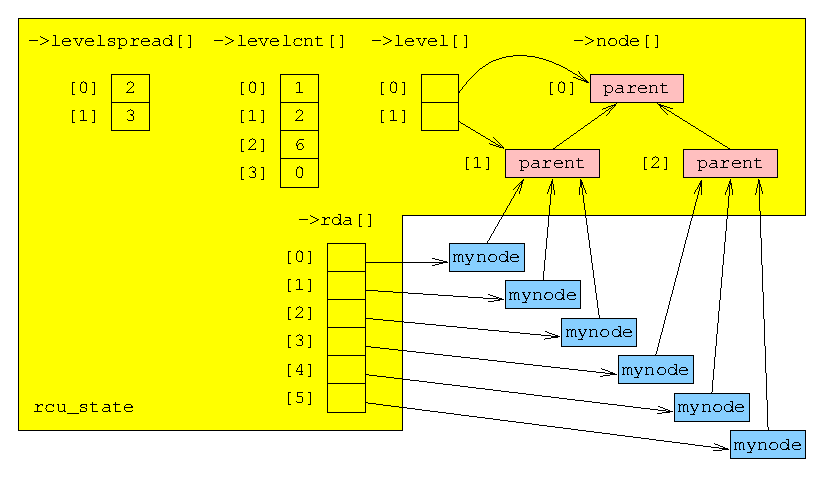
\includegraphics{appendix/rcuimpl/RCUTreeInit}}
\caption{Initialized RCU Data Layout}
\label{fig:app:rcuimpl:rcutree:Initialized RCU Data Layout}
\end{figure*}

This section walks through the initialization code, which links the
main data structures together as shown in
Figure~\ref{fig:app:rcuimpl:rcutree:Initialized RCU Data Layout}.
The yellow region represents fields in the \co{rcu_state} data
structure, including the \co{->node} array, individual elements
of which are shown in pink, matching the convention used in
Section~\ref{app:rcuimpl:rcutree:Hierarchical RCU Overview}.
The blue boxes each represent one \co{rcu_data} structure,
and the group of blue boxes makes up a set of per-CPU \co{rcu_data}
structures.

The \co{->levelcnt[]} array is initialized at compile time, as is
\co{->level[0]}, but the rest of the values and pointers are filled
in by the functions described in the following sections.
The figure shows a two-level hierarchy, but one-level and three-level
hierarchies are possible as well.
Each element of the \co{->levelspread[]} array gives the number of
children per node at the corresponding level of the hierarchy.
In the figure, therefore, the root node has two children and the
nodes at the leaf level each have three children.
Each element of the \co{levelcnt[]} array indicates how many nodes
there are on the corresponding level of the hierarchy: 1 at the root
level, 2 at the leaf level, and 6 at the \co{rcu_data} level---and any
extra elements are unused and left as zero.
Each element of the \co{->level[]} array references the first
node of the corresponding level of the \co{rcu_node} hierarchy,
and each element of the \co{->rda[]} array references the corresponding
CPU's \co{rcu_data} structure.
The \co{->parent} field of each \co{rcu_node} structure references
its parent, except for the root \co{rcu_node} structure, which
has a \co{NULL} \co{->parent} pointer.
Finally, the \co{->mynode} field of each \co{rcu_data} structure
references its parent \co{rcu_node} structure.

\QuickQuiz{}
	How does the code traverse a given path through
	the \co{rcu_node} hierarchy from root to leaves?
\QuickQuizAnswer{
	It turns out that the code never needs to do such a traversal,
	so there is nothing special in place to handle this.
} \QuickQuizEnd

Again, the following sections walk through the code that builds this
structure.

\subsubsection{\tt rcu\_init\_levelspread()}
\label{app:rcuimpl:rcutreewt:rcu-init-levelspread}

\begin{figure}[tbp]
{ \scriptsize
\begin{verbatim}
  1 #ifdef CONFIG_RCU_FANOUT_EXACT
  2 static void __init
  3 rcu_init_levelspread(struct rcu_state *rsp)
  4 {
  5   int i;
  6
  7   for (i = NUM_RCU_LVLS - 1; i >= 0; i--)
  8     rsp->levelspread[i] = CONFIG_RCU_FANOUT;
  9 }
 10 #else
 11 static void __init
 12 rcu_init_levelspread(struct rcu_state *rsp)
 13 {
 14   int ccur;
 15   int cprv;
 16   int i;
 17
 18   cprv = NR_CPUS;
 19   for (i = NUM_RCU_LVLS - 1; i >= 0; i--) {
 20     ccur = rsp->levelcnt[i];
 21     rsp->levelspread[i] = (cprv + ccur - 1) / ccur;
 22     cprv = ccur;
 23   }
 24 }
 25 #endif
\end{verbatim}
}
\caption{{\tt rcu\_init\_levelspread()} Code}
\label{fig:app:rcuimpl:rcutreewt:Code for rcu-init-levelspread}
\end{figure}

Figure~\ref{fig:app:rcuimpl:rcutreewt:Code for rcu-init-levelspread}
shows the code for the \co{rcu_init_levelspread()} function, which controls
the fanout, or the number of children per parent,
in the \co{rcu_node} hierarchy.
There are two versions of this function, one shown on lines~2-9 that
enforces the exact fanout (specified by \co{CONFIG_RCU_FANOUT}),
and the other on lines~11-25 that determines the number of child nodes
based indirectly on the specified fanout, but then balances the tree.
The \co{CONFIG_RCU_FANOUT_EXACT} kernel parameter selects which version
to use for a given kernel build.

The exact-fanout version simply assigns all of the elements of the
specified \co{rcu_state} structure's \co{->levelspread} array to
the \co{CONFIG_RCU_FANOUT} kernel parameter, as shown by the loop
on lines~7 and 8.

The hierarchy-balancing version on lines~11-24
uses a pair of local variables \co{ccur} and \co{cprv} which track
the number of \co{rcu_node} structures on the current and previous
levels, respectively.
This function works from the leaf level up the hierarchy, so \co{cprv}
is initialized by line~18 to \co{NR_CPUS}, which corresponds
to the number of \co{rcu_data} structures that feed into the leaf level.
Lines~19-23 iterate from the leaf to the root.
Within this loop, line~20 picking up
the number of \co{rcu_node} structures for the current level into
\co{ccur}.
Line~21 then rounds up the ratio of the number of nodes on the previous
(lower) level (be they \co{rcu_node} or \co{rcu_data})
to the number of \co{rcu_node} structures on the current
level, placing the result in the specified \co{rcu_state} structure's
\co{->levelspread} array.
Line~22 then sets up for the next pass through the loop.

After a call to either function, the \co{->levelspread} array contains
the number of children for each level of the \co{rcu_node} hierarchy.

\subsubsection{\tt rcu\_init\_one()}
\label{app:rcuimpl:rcutreewt:rcu-init-one}

\begin{figure}[tbp]
{ \scriptsize
\begin{verbatim}
  1 static void __init rcu_init_one(struct rcu_state *rsp)
  2 {
  3   int cpustride = 1;
  4   int i;
  5   int j;
  6   struct rcu_node *rnp;
  7
  8   for (i = 1; i < NUM_RCU_LVLS; i++)
  9     rsp->level[i] = rsp->level[i - 1] +
 10                     rsp->levelcnt[i - 1];
 11   rcu_init_levelspread(rsp);
 12   for (i = NUM_RCU_LVLS - 1; i >= 0; i--) {
 13     cpustride *= rsp->levelspread[i];
 14     rnp = rsp->level[i];
 15     for (j = 0; j < rsp->levelcnt[i]; j++, rnp++) {
 16       spin_lock_init(&rnp->lock);
 17       rnp->qsmask = 0;
 18       rnp->qsmaskinit = 0;
 19       rnp->grplo = j * cpustride;
 20       rnp->grphi = (j + 1) * cpustride - 1;
 21       if (rnp->grphi >= NR_CPUS)
 22         rnp->grphi = NR_CPUS - 1;
 23       if (i == 0) {
 24         rnp->grpnum = 0;
 25         rnp->grpmask = 0;
 26         rnp->parent = NULL;
 27       } else {
 28         rnp->grpnum = j % rsp->levelspread[i - 1];
 29         rnp->grpmask = 1UL << rnp->grpnum;
 30         rnp->parent = rsp->level[i - 1] +
 31                 j / rsp->levelspread[i - 1];
 32       }
 33       rnp->level = i;
 34     }
 35   }
 36 }
\end{verbatim}
}
\caption{{\tt rcu\_init\_one()} Code}
\label{fig:app:rcuimpl:rcutreewt:Code for rcu-init-one}
\end{figure}

Figure~\ref{fig:app:rcuimpl:rcutreewt:Code for rcu-init-one}
shows the code for \co{rcu_init_one()}, which does boot-time initialization
for the specified
\co{rcu_state} structure.

Recall from
Section~\ref{app:rcuimpl:rcutreewt:RCU Global State}
that the \co{->levelcnt[]} array in the \co{rcu_state} structure
is compile-time initialized to the number of nodes at each level of
the hierarchy starting from the root,
with an additional element in the array initialized
to the maximum possible number of CPUs, \co{NR_CPUS}.
In addition, the first element of the \co{->level[]} array is compile-time
initialized to reference to the root \co{rcu_node} structure, which is
in turn
the first element of the \co{->node[]} array in the \co{rcu_state} structure.
This array is further laid out in breadth-first order.
Keeping all of this in mind, the loop at lines~8-10 initializes the rest
of the \co{->level[]} array to reference the first \co{rcu_node} structure
of each level of the \co{rcu_node} hierarchy.

Line~11 then invokes \co{rcu_init_levelspread()}, which fills in the
\co{->levelspread[]} array, as was described in
Section~\ref{app:rcuimpl:rcutreewt:rcu-init-levelspread}.
The auxiliary arrays are then fully initialized, and thus ready for
the loop from lines~15-35, each pass through which initializes
one level of the \co{rcu_node} hierarchy, starting from the leaves.

Line~13 computes the number of CPUs per \co{rcu_node} structure for
the current level of the hierarchy, and line~14 obtains a pointer
to the first \co{rcu_node} structure on the current level of the
hierarchy, in preparation for the loop from lines~15-34, each pass
through which initializes one \co{rcu_node} structure.

Lines~16-18 initialize the \co{rcu_node} structure's spinlock and
its CPU masks.
The \co{qsmaskinit} field will have bits set as CPUs come online
later in boot, and the \co{qsmask} field will have bits set
when the first grace period starts.
Line~19 sets the \co{->grplo} field to the number of the this
\co{rcu_node} structure's first CPU and line~20 sets the
\co{->grphi} to the number of this \co{rcu_node} structure's
last CPU.
If the last \co{rcu_node} structure on a given level of the
hierarchy is only partially full, lines~21 and 22 set its
\co{->grphi} field to the number of the last possible CPU in the system.

Lines~24-26 initialize the \co{->grpnum}, \co{->grpmask}, and
\co{->parent} fields for the root \co{rcu_node} structure, which
has no parent, hence the zeroes and NULL.
Lines~28-31 initialize these same fields for the rest of the
\co{rcu_node} structures in the hierarchy.
Line~28 computes the \co{->grpnum} field as the index of this
\co{rcu_node} structure within
the set having the same parent, and
line~29 sets the corresponding bit in the \co{->grpmask} field.
Finally, lines~30-31 places a pointer to the parent node into the
\co{->parent} field.
These three fields will used to propagate quiescent states up the
hierarchy.

Finally, line~33 records the hierarchy level in \co{->level},
which is used for tracing when traversing the full hierarchy.

\subsubsection{\tt \_\_rcu\_init()}
\label{app:rcuimpl:rcutreewt:rcu-init}

\begin{figure}[tbp]
{ \scriptsize
\begin{verbatim}
  1 #define RCU_DATA_PTR_INIT(rsp, rcu_data) \
  2 do { \
  3   rnp = (rsp)->level[NUM_RCU_LVLS - 1]; \
  4   j = 0; \
  5   for_each_possible_cpu(i) { \
  6     if (i > rnp[j].grphi) \
  7       j++; \
  8     per_cpu(rcu_data, i).mynode = &rnp[j]; \
  9     (rsp)->rda[i] = &per_cpu(rcu_data, i); \
 10   } \
 11 } while (0)
 12
 13 void __init __rcu_init(void)
 14 {
 15   int i;
 16   int j;
 17   struct rcu_node *rnp;
 18
 19   rcu_init_one(&rcu_state);
 20   RCU_DATA_PTR_INIT(&rcu_state, rcu_data);
 21   rcu_init_one(&rcu_bh_state);
 22   RCU_DATA_PTR_INIT(&rcu_bh_state, rcu_bh_data);
 23
 24   for_each_online_cpu(i)
 25     rcu_cpu_notify(&rcu_nb, CPU_UP_PREPARE,
 26                    (void *)(long)i);
 27   register_cpu_notifier(&rcu_nb);
 28 }
\end{verbatim}
}
\caption{{\tt \_\_rcu\_init()} Code}
\label{fig:app:rcuimpl:rcutreewt:Code for rcu-init}
\end{figure}

Figure~\ref{fig:app:rcuimpl:rcutreewt:Code for rcu-init}
shows the \co{__rcu_init()} function and its \co{RCU_DATA_PTR_INIT()}
helper macro.
The \co{__rcu_init()} function is invoked during early boot,
before the scheduler has initialized, and before more than one
CPU is running.

The \co{RCU_DATA_PTR_INIT()} macro takes as arguments a pointer to
an \co{rcu_state} structure and the name of a set of \co{rcu_data}
per-CPU variables.
This macro scans the per-CPU \co{rcu_data}
structures, assigning the \co{->mynode} pointer of each \co{rcu_data}
structure to point to the corresponding leaf \co{rcu_node} structure.
It also fills out the specified \co{rcu_state} structure's
\co{->rda[]} array entries to each point to the corresponding
\co{rcu_data} structure.
Line~3 picks up a pointer to the first leaf \co{rcu_node} structure
in local variable \co{rnp} (which must be declared by the invoker of
this macro),
and line~4 sets local variable \co{j} to the corresponding leaf-node
number of zero.
Each pass through the loop spanning lines~5-10 performs initialization
for the corresponding potential CPU (as specified by \co{NR_CPUS}).
Within this loop, line~6 checks to see if we have moved beyond the
bounds of the current leaf \co{rcu_node} structure, and, if so,
line~7 advances to the next structure.
Then, still within the loop, line~8 sets the \co{->mynode} pointer
of the current CPU's \co{rcu_data} structure to reference the current
leaf \co{rcu_node} structure, and line~9 sets the current CPU's \co{->rda[]}
element (within the \co{rcu_state} structure) to reference the
current CPU's \co{rcu_data} structure.

\QuickQuiz{}
	C-preprocessor macros are \emph{so} 1990s!
	Why not get with the times and convert \co{RCU_DATA_PTR_INIT()}
	in Figure~\ref{fig:app:rcuimpl:rcutreewt:Code for rcu-init}
	to be a function?
\QuickQuizAnswer{
	Because, although it is possible to pass a reference to
	a particular CPU's instance of a per-CPU variable to a function,
	there does not appear to be a good way pass a reference to
	the full set of instances of a given per-CPU variable to
	a function.
	One could of course build an array of pointers, then pass a
	reference to the array in, but that is part of what
	the \co{RCU_DATA_PTR_INIT()} macro is doing in the first place.
} \QuickQuizEnd

The \co{__rcu_init()} function first invokes \co{rcu_init_one()}
on the \co{rcu_state} structure on line~19, then invokes
\co{RCU_DATA_PTR_INIT()} on the \co{rcu_state} structure and
the \co{rcu_data} set of per-CPU variables.
It then repeats this for \co{rcu_bh_state} and \co{rcu_bh_data}
on lines~21-22.
The loop spanning lines~24-26 invokes \co{rcu_cpu_notify()} for
each CPU that is currently online (which should be only the boot
CPU), and line~27 registers a notifier so that \co{rcu_cpu_notify()}
will be invoked each time a CPU comes online, in order to inform
RCU of its presence.

\QuickQuiz{}
	What happens if a CPU comes online between the time
	that the last online CPU is notified on lines~25-26 of
	Figure~\ref{fig:app:rcuimpl:rcutreewt:Code for rcu-init}
	and the time that \co{register_cpu_notifier()} is invoked
	on line~27?
\QuickQuizAnswer{
	Only one CPU is online at this point, so the only way another
	CPU can come online is if this CPU puts it online, which it
	is not doing.
} \QuickQuizEnd

The \co{rcu_cpu_notify()} and related functions are discussed in
Section~\ref{app:rcuimpl:rcutreewt:CPU Hotplug}
below.

\subsection{CPU Hotplug}
\label{app:rcuimpl:rcutreewt:CPU Hotplug}

The CPU-hotplug functions described in the following sections
allow RCU to track which CPUs are and are not present, but also
complete initialization of each CPU's \co{rcu_data} structure
as that CPU comes online.

\subsubsection{\tt rcu\_init\_percpu\_data()}
\label{app:rcuimpl:rcutreewt:rcu-init-percpu-data}

\begin{figure}[tbp]
{ \scriptsize
\begin{verbatim}
  1 static void
  2 rcu_init_percpu_data(int cpu, struct rcu_state *rsp)
  3 {
  4   unsigned long flags;
  5   int i;
  6   long lastcomp;
  7   unsigned long mask;
  8   struct rcu_data *rdp = rsp->rda[cpu];
  9   struct rcu_node *rnp = rcu_get_root(rsp);
 10
 11   spin_lock_irqsave(&rnp->lock, flags);
 12   lastcomp = rsp->completed;
 13   rdp->completed = lastcomp;
 14   rdp->gpnum = lastcomp;
 15   rdp->passed_quiesc = 0;
 16   rdp->qs_pending = 1;
 17   rdp->beenonline = 1;
 18   rdp->passed_quiesc_completed = lastcomp - 1;
 19   rdp->grpmask = 1UL << (cpu - rdp->mynode->grplo);
 20   rdp->nxtlist = NULL;
 21   for (i = 0; i < RCU_NEXT_SIZE; i++)
 22     rdp->nxttail[i] = &rdp->nxtlist;
 23   rdp->qlen = 0;
 24   rdp->blimit = blimit;
 25 #ifdef CONFIG_NO_HZ
 26   rdp->dynticks = &per_cpu(rcu_dynticks, cpu);
 27 #endif /* #ifdef CONFIG_NO_HZ */
 28   rdp->cpu = cpu;
 29   spin_unlock(&rnp->lock);
 30   spin_lock(&rsp->onofflock);
 31   rnp = rdp->mynode;
 32   mask = rdp->grpmask;
 33   do {
 34     spin_lock(&rnp->lock);
 35     rnp->qsmaskinit |= mask;
 36     mask = rnp->grpmask;
 37     spin_unlock(&rnp->lock);
 38     rnp = rnp->parent;
 39   } while (rnp != NULL && !(rnp->qsmaskinit & mask));
 40   spin_unlock(&rsp->onofflock);
 41   cpu_quiet(cpu, rsp, rdp, lastcomp);
 42   local_irq_restore(flags);
 43 }
\end{verbatim}
}
\caption{{\tt rcu\_init\_percpu\_data()} Code}
\label{fig:app:rcuimpl:rcutreewt:Code for rcu-init-percpu-data}
\end{figure}

Figure~\ref{fig:app:rcuimpl:rcutreewt:Code for rcu-init-percpu-data}
shows the code for \co{rcu_init_percpu_data()}, which initializes
the specified CPU's \co{rcu_data} structure in response to booting
up or to that CPU coming online.
It also sets up the \co{rcu_node} hierarchy so that this CPU will
participate in future grace periods.

Line~8 gets a pointer to this CPU's \co{rcu_data} structure, based
on the specified \co{rcu_state} structure, and places this pointer
into the local variable \co{rdp}.
Line~9 gets a pointer to the root \co{rcu_node} structure for the
specified \co{rcu_state} structure, placing it in local variable
\co{rnp}.

Lines~11-29 initialize the fields of the \co{rcu_data} structure
under the protection of the root \co{rcu_node} structure's lock
in order to ensure consistent values.
Line~17 is important for tracing, due to the fact that many Linux
distributions set \co{NR_CPUS} to a very large number, which could
result in excessive output when tracing \co{rcu_data} structures.
The \co{->beenonline} field is used to solve this problem, as
it will be set to the value one on any \co{rcu_data} structure
corresponding to a CPU that has ever been online, and set to zero
for all other \co{rcu_data} structures.
This allows the tracing code to easily ignore irrelevant CPUs.

Lines~30-40 propagate the onlining CPU's bit up the \co{rcu_node}
hierarchy, proceeding until either the root \co{rcu_node} is
reached or until the corresponding bit is already set, whichever
comes first.
This bit-setting is done under the protection of \co{->onofflock}
in order to exclude initialization of a new grace period, and, in addition,
each \co{rcu_node} structure is initialized under the protection
of its lock.
Line~41 then invokes \co{cpu_quiet()} to signal RCU that this
CPU has been in an extended quiescent state, and finally, line~42
re-enables irqs.

\QuickQuiz{}
	Why call \co{cpu_quiet()} on line~41 of
	Figure~\ref{fig:app:rcuimpl:rcutreewt:Code for rcu-init-percpu-data},
	given that we are excluding grace periods with various
	locks, and given that any earlier grace periods would not have
	been waiting on this previously-offlined CPU?
\QuickQuizAnswer{
	A new grace period might have started just after the
	\co{->onofflock} was released on line~40.
	The \co{cpu_quiet()} will help expedite such a grace period.
} \QuickQuizEnd

It is important to note that \co{rcu_init_percpu_data()} is invoked
not only at boot time, but also every time that a given CPU is brought
online.

\subsubsection{\tt rcu\_online\_cpu()}
\label{app:rcuimpl:rcutreewt:rcu-online-cpu}

\begin{figure}[tbp]
{ \scriptsize
\begin{verbatim}
  1 static void __cpuinit rcu_online_cpu(int cpu)
  2 {
  3 #ifdef CONFIG_NO_HZ
  4   struct rcu_dynticks *rdtp;
  5
  6   rdtp = &per_cpu(rcu_dynticks, cpu);
  7   rdtp->dynticks_nesting = 1;
  8   rdtp->dynticks |= 1;
  9   rdtp->dynticks_nmi = (rdtp->dynticks_nmi + 1) & ~0x1;
 10 #endif /* #ifdef CONFIG_NO_HZ */
 11   rcu_init_percpu_data(cpu, &rcu_state);
 12   rcu_init_percpu_data(cpu, &rcu_bh_state);
 13   open_softirq(RCU_SOFTIRQ, rcu_process_callbacks);
 14 }
\end{verbatim}
}
\caption{{\tt rcu\_online\_cpu()} Code}
\label{fig:app:rcuimpl:rcutreewt:Code for rcu-online-cpu}
\end{figure}

Figure~\ref{fig:app:rcuimpl:rcutreewt:Code for rcu-online-cpu}
shows the code for \co{rcu_online_cpu()}, which informs RCU that the
specified CPU is coming online.

When dynticks (\co{CONFIG_NO_HZ}) is enabled, line~6 obtains a
reference to the specified CPU's \co{rcu_dynticks} structure, which
is shared between the ``rcu'' and ``rcu\_bh'' implementations of RCU.
Line~7 sets the \co{->dynticks_nesting} field to the value one,
reflecting the fact that a newly onlined CPU is not in dynticks-idle
mode (recall that the \co{->dynticks_nesting} field tracks the
number of reasons that the corresponding CPU needs to be tracked for
RCU read-side critical sections, in this case because it can run
process-level code).
Line~8 forces the \co{->dynticks} field to an odd value that is
at least as large as the last value it had when previously online,
again reflecting the fact that newly onlined CPUs are not in dynticks-idle
mode, and line~9 forces the \co{->dynticks_nmi} field to an even value
that is at least as large as the last value it had when previously
online, reflecting the fact that this CPU is not currently executing
in an NMI handler.

Lines~11-13 are executed regardless of the value of the
\co{CONFIG_NO_HZ} kernel parameter.
Line~11 initializes the specified CPU's \co{rcu_data} structure
for ``rcu'', and line~12 does so for ``rcu\_bh''.
Finally, line~13 registers the \co{rcu_process_callbacks()} to be
invoked by subsequent \co{raise_softirq()} invocations on this CPU.

\subsubsection{\tt rcu\_offline\_cpu()}
\label{app:rcuimpl:rcutreewt:rcu-offline-cpu}

\begin{figure}[tbp]
{ \scriptsize
\begin{verbatim}
  1 static void
  2 __rcu_offline_cpu(int cpu, struct rcu_state *rsp)
  3 {
  4   int i;
  5   unsigned long flags;
  6   long lastcomp;
  7   unsigned long mask;
  8   struct rcu_data *rdp = rsp->rda[cpu];
  9   struct rcu_data *rdp_me;
 10   struct rcu_node *rnp;
 11
 12   spin_lock_irqsave(&rsp->onofflock, flags);
 13   rnp = rdp->mynode;
 14   mask = rdp->grpmask;
 15   do {
 16     spin_lock(&rnp->lock);
 17     rnp->qsmaskinit &= ~mask;
 18     if (rnp->qsmaskinit != 0) {
 19       spin_unlock(&rnp->lock);
 20       break;
 21     }
 22     mask = rnp->grpmask;
 23     spin_unlock(&rnp->lock);
 24     rnp = rnp->parent;
 25   } while (rnp != NULL);
 26   lastcomp = rsp->completed;
 27   spin_unlock(&rsp->onofflock);
 28   cpu_quiet(cpu, rsp, rdp, lastcomp);
 29   rdp_me = rsp->rda[smp_processor_id()];
 30   if (rdp->nxtlist != NULL) {
 31     *rdp_me->nxttail[RCU_NEXT_TAIL] = rdp->nxtlist;
 32     rdp_me->nxttail[RCU_NEXT_TAIL] =
 33         rdp->nxttail[RCU_NEXT_TAIL];
 34     rdp->nxtlist = NULL;
 35     for (i = 0; i < RCU_NEXT_SIZE; i++)
 36       rdp->nxttail[i] = &rdp->nxtlist;
 37     rdp_me->qlen += rdp->qlen;
 38     rdp->qlen = 0;
 39   }
 40   local_irq_restore(flags);
 41 }
 42
 43 static void rcu_offline_cpu(int cpu)
 44 {
 45   __rcu_offline_cpu(cpu, &rcu_state);
 46   __rcu_offline_cpu(cpu, &rcu_bh_state);
 47 }
\end{verbatim}
}
\caption{{\tt rcu\_offline\_cpu()} Code}
\label{fig:app:rcuimpl:rcutreewt:Code for rcu-offline-cpu}
\end{figure}

Figure~\ref{fig:app:rcuimpl:rcutreewt:Code for rcu-offline-cpu}
shows the code for \co{__rcu_offline_cpu()} and its wrapper
function, \co{rcu_offline_cpu()}.
The purpose of this wrapper function (shown in lines~43-47 of the figure)
is simply to invoke \co{__rcu_offline_cpu()} twice, once for ``rcu'' and
again for ``rcu\_bh''.
The purpose of the \co{__rcu_offline_cpu()} function is to
prevent future grace periods from waiting on the CPU being offlined,
to note the extended quiescent state, and to find a new home for
any RCU callbacks in process on this CPU.

Turning to \co{__rcu_offline_cpu()}, shown on lines~1-41 of the figure,
line~12 acquires the specified \co{rcu_state} structure's
\co{->onofflock}, excluding grace-period initialization for
multi-\co{rcu_node} hierarchies.

\QuickQuiz{}
	But what if the \co{rcu_node} hierarchy has only a single
	structure, as it would on a small system?
	What prevents concurrent grace-period initialization in that
	case, given the code in
	Figure~\ref{fig:app:rcuimpl:rcutreewt:Code for rcu-offline-cpu}?
\QuickQuizAnswer{
	The later acquisition of the sole \co{rcu_node} structure's
	\co{->lock} on line~16 excludes grace-period initialization,
	which must acquire this same lock in order to initialize this
	sole \co{rcu_node} structure for the new grace period.

	The \co{->onofflock} is needed only for multi-node hierarchies,
	and is used in that case as an alternative to acquiring and
	holding \emph{all} of the \co{rcu_node} structures'
	\co{->lock} fields, which would be incredibly painful on
	large systems.
} \QuickQuizEnd

Line~13 picks up a pointer to the leaf \co{rcu_node} structure corresponding
to this CPU, using the \co{->mynode} pointer in this CPU's \co{rcu_data}
structure
(see Figure~\ref{fig:app:rcuimpl:rcutree:Initialized RCU Data Layout}).
Line~14 picks up a mask with this CPU's bit set for use on
the leaf \co{rcu_node} structure's \co{qsmask} field.

The loop spanning lines~15-25 then clears this CPU's bits up the
\co{rcu_node} hierarchy, starting with this CPU's leaf \co{rcu_node}
structure.
Line~16 acquires the current \co{rcu_node} structure's \co{->lock}
field, and line~17 clears the bit corresponding to this CPU
(or group, higher up in the hierarchy) from the \co{->qsmaskinit}
field, so that future grace periods will not wait on quiescent states
from this CPU.
If the resulting \co{->qsmaskinit} value is non-zero, as checked by
line~18, then the
current \co{rcu_node} structure has other online CPUs that it
must track, so line~19 releases the current \co{rcu_node} structure's
\co{->lock} and line~20 exits the loop.
Otherwise, we need to continue walking up the \co{rcu_node} hierarchy.
In this case, line~22 picks up the mask to apply to the next level up,
line~23 releases the current \co{rcu_node} structure's \co{->lock},
and line~24 advances up to the next level of the hierarchy.
Line~25 exits the loop should we exit out the top of the hierarchy.

\QuickQuiz{}
	But does line~25 of
	Figure~\ref{fig:app:rcuimpl:rcutreewt:Code for rcu-offline-cpu}
	ever really exit the loop?
	Why or why not?
\QuickQuizAnswer{
	The only way that line~25 could exit the loop is if \emph{all}
	CPUs were to be put offline.
	This cannot happen in the Linux kernel as of 2.6.28, though
	other environments have been designed to offline all CPUs
	during the normal shutdown procedure.
} \QuickQuizEnd

Line~26 picks up the specified \co{rcu_state} structure's
\co{->completed} field into the local variable \co{lastcomp},
line~27 releases \co{->onofflock} (but leaves irqs disabled),
and line~28 invokes \co{cpu_quiet()} in order to note that the
CPU being offlined is now in an extended quiescent state, passing
in \co{lastcomp} to avoid reporting this quiescent state against
a different grace period than it occurred in.

\QuickQuiz{}
	Suppose that line~26 got executed seriously out of order in
	Figure~\ref{fig:app:rcuimpl:rcutreewt:Code for rcu-offline-cpu},
	so that \co{lastcomp} is set to some prior grace period, but
	so that the current grace period is still waiting on the
	now-offline CPU?
	In this case, won't the call to \co{cpu_quiet()} fail to
	report the quiescent state, thus causing the grace period
	to wait forever for this now-offline CPU?
\QuickQuizAnswer{
	First, the lock acquisitions on lines~16 and 12 would prevent
	the execution of line~26 from being pushed that far out of
	order.
	Nevertheless, even if line~26 managed to be misordered that
	dramatically, what would happen is that \co{force_quiescent_state()}
	would eventually be invoked, and would notice that the current
	grace period was waiting for a quiescent state from an offline
	CPU.
	Then \co{force_quiescent_state()} would report the extended
	quiescent state on behalf of the offlined CPU.
} \QuickQuizEnd

\QuickQuiz{}
	Given that an offline CPU is in an extended quiescent state,
	why does line~28 of
	Figure~\ref{fig:app:rcuimpl:rcutreewt:Code for rcu-offline-cpu}
	need to care which grace period it is
	dealing with?
\QuickQuizAnswer{
	It really does not need to care in this case.
	However, because it \emph{does} need to care in many other
	cases, the \co{cpu_quiet()} function does take the
	grace-period number as an argument, so some value must be
	supplied.
} \QuickQuizEnd

Lines~29-39 move any RCU callbacks from the CPU going offline to the
currently running CPU.
This operation must avoid reordering the callbacks being moved, as
otherwise \co{rcu_barrier()} will not work correctly.
Line~29 puts a pointer to the currently running CPU's \co{rcu_data}
structure into local variable \co{rdp_me}.
Line~30 then checks to see if the CPU going offline has any RCU callbacks.
If so, lines~31-38 move them.
Line~31 splices the list of callbacks onto the end of the running CPU's
list.
Lines~32-33 sets the running CPU's callback tail pointer to that of
the CPU going offline, and then lines 34-36 initialize the going-offline
CPU's list to be empty.
Line~37 adds the length of the going-offline CPU's callback list to
that of the currently running CPU, and, finally, line 38 zeroes the
going-offline CPU's list length.

\QuickQuiz{}
	But this list movement in
	Figure~\ref{fig:app:rcuimpl:rcutreewt:Code for rcu-offline-cpu}
	makes all of the going-offline CPU's callbacks go through
	another grace period, even if they were ready to invoke.
	Isn't that inefficient?
	Furthermore, couldn't an unfortunate pattern of CPUs going
	offline then coming back online prevent a given callback from
	ever being invoked?
\QuickQuizAnswer{
	It is inefficient, but it is simple.
	Given that this is not a commonly executed code path, this
	is the right tradeoff.
	The starvation case would be a concern, except that the
	online and offline process involves multiple grace periods.
} \QuickQuizEnd

Finally, line~40 re-enables irqs.

\subsection{Miscellaneous Functions}
\label{app:rcuimpl:rcutreewt:Miscellaneous Functions}

This section describes the miscellaneous utility functions:
\begin{enumerate}
\item	\co{rcu_batches_completed}
\item	\co{rcu_batches_completed_bh}
\item	\co{cpu_has_callbacks_ready_to_invoke}
\item	\co{cpu_needs_another_gp}
\item	\co{rcu_get_root}
\end{enumerate}

\begin{figure}[tbp]
{ \scriptsize
\begin{verbatim}
  1 long rcu_batches_completed(void)
  2 {
  3   return rcu_state.completed;
  4 }
  5
  6 long rcu_batches_completed_bh(void)
  7 {
  8   return rcu_bh_state.completed;
  9 }
 10
 11 static int
 12 cpu_has_callbacks_ready_to_invoke(struct rcu_data *rdp)
 13 {
 14   return &rdp->nxtlist != rdp->nxttail[RCU_DONE_TAIL];
 15 }
 16
 17 static int
 18 cpu_needs_another_gp(struct rcu_state *rsp,
 19                      struct rcu_data *rdp)
 20 {
 21   return *rdp->nxttail[RCU_DONE_TAIL] &&
 22          ACCESS_ONCE(rsp->completed) ==
 23          ACCESS_ONCE(rsp->gpnum);
 24 }
 25
 26 static struct rcu_node
 27 *rcu_get_root(struct rcu_state *rsp)
 28 {
 29   return &rsp->node[0];
 30 }
\end{verbatim}
}
\caption{Miscellaneous Functions}
\label{fig:app:rcuimpl:rcutreewt:Miscellaneous Functions}
\end{figure}

Figure~\ref{fig:app:rcuimpl:rcutreewt:Miscellaneous Functions}
shows a number of miscellaneous functions.
Lines~1-9 show \co{rcu_batches_completed()} and
\co{rcu_batches_completed_bh()}, which are used by the rcutorture
test suite.
Lines~11-15 show \co{cpu_has_callbacks_ready_to_invoke()}, which
indicates whether the specified \co{rcu_data} structure has RCU
callbacks that have passed through their grace period, which
is indicated by the ``done'' tail pointer no longer pointing
to the head of the list.
Lines~17-24 show \co{cpu_needs_another_gp()}, which indicates
whether the CPU corresponding to the specified \co{rcu_data}
structure requires an additional grace period during a time when
no grace period is in progress.
Note that the specified \co{rcu_data} structure is required
to be associated with the specified \co{rcu_state} structure.
Finally, lines~26-30 show \co{rcu_get_root()}, which returns
the root \co{rcu_node} structure associated with the specified
\co{rcu_state} structure.

\subsection{Grace-Period-Detection Functions}
\label{app:rcuimpl:rcutreewt:Grace-Period-Detection Functions}

This section covers functions that are directly involved in detecting
beginnings and ends of grace periods.
This of course includes actually starting and ending grace periods,
but also includes noting when other CPUs have started or ended
grace periods.

\subsubsection{Noting New Grace Periods}
\label{app:rcuimpl:rcutreewt:Noting New Grace Periods}

The main purpose of Hierarchical RCU is to detect grace periods,
and the functions more directly involved in this task are described
in this section.
Section~\ref{app:rcuimpl:rcutreewt:Noting New Grace Periods}
covers functions that allow CPUs to note that a new grace period has
begun,
Section~\ref{app:rcuimpl:rcutreewt:Noting End of Old Grace Periods}
covers functions that allow CPUs to note that an existing grace period
has ended,
Section~\ref{app:rcuimpl:rcutreewt:Starting a Grace Period}
covers \co{rcu_start_gp()}, which starts a new grace period, and
Section~\ref{app:rcuimpl:rcutreewt:Reporting Quiescent States}
covers functions involved in reporting CPUs' quiescent states to
the RCU core.

\begin{figure}[tbp]
{ \scriptsize
\begin{verbatim}
  1 static void note_new_gpnum(struct rcu_state *rsp,
  2                            struct rcu_data *rdp)
  3 {
  4   rdp->qs_pending = 1;
  5   rdp->passed_quiesc = 0;
  6   rdp->gpnum = rsp->gpnum;
  7   rdp->n_rcu_pending_force_qs = rdp->n_rcu_pending +
  8               RCU_JIFFIES_TILL_FORCE_QS;
  9 }
 10
 11 static int
 12 check_for_new_grace_period(struct rcu_state *rsp,
 13                            struct rcu_data *rdp)
 14 {
 15   unsigned long flags;
 16   int ret = 0;
 17
 18   local_irq_save(flags);
 19   if (rdp->gpnum != rsp->gpnum) {
 20     note_new_gpnum(rsp, rdp);
 21     ret = 1;
 22   }
 23   local_irq_restore(flags);
 24   return ret;
 25 }
\end{verbatim}
}
\caption{Noting New Grace Periods}
\label{fig:app:rcuimpl:rcutreewt:Noting New Grace Periods}
\end{figure}

Figure~\ref{fig:app:rcuimpl:rcutreewt:Noting New Grace Periods}
shows the code for \co{note_new_gpnum()}, which updates state to reflect
a new grace period, as well as \co{check_for_new_grace_period()}, which
is used by CPUs to detect when other CPUs have started a new grace period.

Line~4 of \co{note_new_gpnum()} sets the \co{->qs_pending} flag is
the current CPU's \co{rcu_data} structure to indicate that RCU needs
a quiescent state from this CPU, line~5 clears the \co{->passed_quiesc}
flag to indicate that this CPU has not yet passed through such a
quiescent state,
line~6 copies the grace-period number from the global \co{rcu_state}
structure to this CPU's \co{rcu_data} structure so that this CPU will
remember that it has already noted the beginning of this new grace
period.
Finally, lines~7-8 record the time in jiffies at which this CPU
will attempt to force holdout CPUs to pass through quiescent states
(by invoking \co{force_quiescent_state()} on or after that future time),
assuming that the grace period does not end beforehand.

Lines~18 and 23 of \co{check_for_new_grace_period()} disable and
re-enable interrupts, respectively.
Line~19 checks to see if there is a new grace period that the current
CPU has not yet noted, and, if so, line~20 invokes \co{note_new_gpnum()}
in order to note the new grace period, and line~21 sets the return value
accordingly.
Either way, line~24 returns status: non-zero if a new grace period has
started, and zero otherwise.

\QuickQuiz{}
	Why not just expand \co{note_new_gpnum()} inline into
	\co{check_for_new_grace_period()} in
	Figure~\ref{fig:app:rcuimpl:rcutreewt:Noting New Grace Periods}?
\QuickQuizAnswer{
	Because \co{note_new_gpnum()} must be called for each new
	grace period, including both those started by this CPU and
	those started by other CPUs.
	In contrast, \co{check_for_new_grace_period()} is called only
	for the case where some other CPU started the grace period.
} \QuickQuizEnd

\subsubsection{Noting End of Old Grace Periods}
\label{app:rcuimpl:rcutreewt:Noting End of Old Grace Periods}

\begin{figure}[tbp]
{ \scriptsize
\begin{verbatim}
  1 static void
  2 rcu_process_gp_end(struct rcu_state *rsp,
  3                    struct rcu_data *rdp)
  4 {
  5   long completed_snap;
  6   unsigned long flags;
  7
  8   local_irq_save(flags);
  9   completed_snap = ACCESS_ONCE(rsp->completed);
 10   if (rdp->completed != completed_snap) {
 11     rdp->nxttail[RCU_DONE_TAIL] =
 12         rdp->nxttail[RCU_WAIT_TAIL];
 13     rdp->nxttail[RCU_WAIT_TAIL] =
 14         rdp->nxttail[RCU_NEXT_READY_TAIL];
 15     rdp->nxttail[RCU_NEXT_READY_TAIL] =
 16         rdp->nxttail[RCU_NEXT_TAIL];
 17     rdp->completed = completed_snap;
 18   }
 19   local_irq_restore(flags);
 20 }
\end{verbatim}
}
\caption{Noting End of Old Grace Periods}
\label{fig:app:rcuimpl:rcutreewt:Noting End of Old Grace Periods}
\end{figure}

\begin{figure}[tb]
\centering
\resizebox{3in}{!}{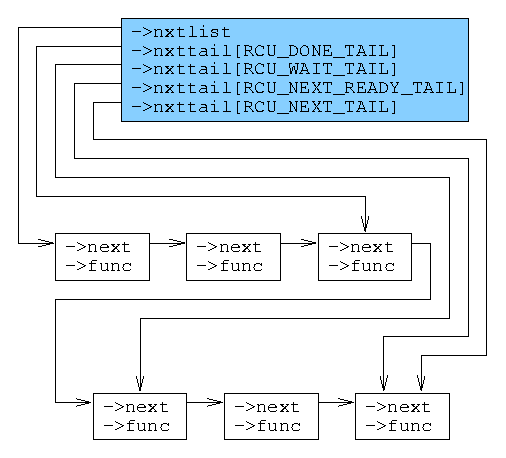
\includegraphics{appendix/rcuimpl/AdvanceRCUCallbacks}}
\caption{RCU Callback List}
\label{fig:app:rcuimpl:rcutree:RCU Callback List}
\end{figure}

Figure~\ref{fig:app:rcuimpl:rcutreewt:Noting End of Old Grace Periods}
shows \co{rcu_process_gp_end()}, which is invoked when a CPU suspects
that a grace period might have ended (possibly because the CPU in question
in fact ended the grace period).
If a grace period really has ended, then this function advances the
current CPU's RCU callbacks, which are managed as a singly linked
list with multiple tail pointers, as shown in
Figure~\ref{fig:app:rcuimpl:rcutree:RCU Callback List}.
This multiple tail pointer layout, spearheaded by
Lai Jiangshan, simplifies list
handling~\cite{LaiJiangshan2008NewClassicAlgorithm}.
In this figure, the blue box represents one CPU's \co{rcu_data}
structure, with the six white boxes at the bottom of the diagram
representing a list of six RCU callbacks (\co{rcu_head} structures).
In this list, the first three callbacks have passed through their
grace period and are thus waiting to be invoked, the fourth
callback (the first on the second line) is waiting for the current
grace period to complete, and the last two are waiting for the
next grace period.
The last two tail pointers reference the last element, so that the
final sublist, which would comprise callbacks that had not yet been
associated with a specific grace period, is empty.

Lines~8 and 19 of
Figure~\ref{fig:app:rcuimpl:rcutreewt:Noting End of Old Grace Periods}
suppress and re-enable interrupts, respectively.
Line~9 picks up a snapshot of the \co{rcu_state} structure's
\co{->completed} field, storing it in the local variable
\co{completed_snap}.
Line~10 checks to see if the current CPU is not yet aware of the
end of a grace period, and if it is not aware,
lines~11-16 advance this CPU's RCU callbacks by manipulating the
tail pointers.
Line~17 then records the most recently completed grace period number
in this CPU's \co{rcu_data} structure in the \co{->completed}
field.

\subsubsection{Starting a Grace Period}
\label{app:rcuimpl:rcutreewt:Starting a Grace Period}

\begin{figure}[tbp]
{ \scriptsize
\begin{verbatim}
  1 static void
  2 rcu_start_gp(struct rcu_state *rsp, unsigned long flags)
  3   __releases(rcu_get_root(rsp)->lock)
  4 {
  5   struct rcu_data *rdp = rsp->rda[smp_processor_id()];
  6   struct rcu_node *rnp = rcu_get_root(rsp);
  7   struct rcu_node *rnp_cur;
  8   struct rcu_node *rnp_end;
  9
 10   if (!cpu_needs_another_gp(rsp, rdp)) {
 11     spin_unlock_irqrestore(&rnp->lock, flags);
 12     return;
 13   }
 14   rsp->gpnum++;
 15   rsp->signaled = RCU_GP_INIT;
 16   rsp->jiffies_force_qs = jiffies +
 17       RCU_JIFFIES_TILL_FORCE_QS;
 18   rdp->n_rcu_pending_force_qs = rdp->n_rcu_pending +
 19       RCU_JIFFIES_TILL_FORCE_QS;
 20   record_gp_stall_check_time(rsp);
 21   dyntick_record_completed(rsp, rsp->completed - 1);
 22   note_new_gpnum(rsp, rdp);
 23   rdp->nxttail[RCU_NEXT_READY_TAIL] =
 24       rdp->nxttail[RCU_NEXT_TAIL];
 25   rdp->nxttail[RCU_WAIT_TAIL] =
 26       rdp->nxttail[RCU_NEXT_TAIL];
 27   if (NUM_RCU_NODES == 1) {
 28     rnp->qsmask = rnp->qsmaskinit;
 29     spin_unlock_irqrestore(&rnp->lock, flags);
 30     return;
 31   }
 32   spin_unlock(&rnp->lock);
 33   spin_lock(&rsp->onofflock);
 34   rnp_end = rsp->level[NUM_RCU_LVLS - 1];
 35   rnp_cur = &rsp->node[0];
 36   for (; rnp_cur < rnp_end; rnp_cur++)
 37     rnp_cur->qsmask = rnp_cur->qsmaskinit;
 38   rnp_end = &rsp->node[NUM_RCU_NODES];
 39   rnp_cur = rsp->level[NUM_RCU_LVLS - 1];
 40   for (; rnp_cur < rnp_end; rnp_cur++) {
 41     spin_lock(&rnp_cur->lock);
 42     rnp_cur->qsmask = rnp_cur->qsmaskinit;
 43     spin_unlock(&rnp_cur->lock);
 44   }
 45   rsp->signaled = RCU_SIGNAL_INIT;
 46   spin_unlock_irqrestore(&rsp->onofflock, flags);
 47 }
\end{verbatim}
}
\caption{Starting a Grace Period}
\label{fig:app:rcuimpl:rcutreewt:Starting a Grace Period}
\end{figure}

Figure~\ref{fig:app:rcuimpl:rcutreewt:Starting a Grace Period}
shows \co{rcu_start_gp()}, which starts a new grace period,
also releasing the root \co{rcu_node} structure's lock, which
must be acquired by the caller.

Line~3 is annotation for the \co{sparse} utility, indicating
that \co{rcu_start_gp()} releases the root \co{rcu_node}
structure's lock.
Local variable \co{rdp} references the running CPU's \co{rcu_data}
structure, \co{rnp} references the root \co{rcu_node} structure,
and \co{rnp_cur} and \co{rnp_end} are used as cursors in traversing
the \co{rcu_node} hierarchy.

Line~10 invokes \co{cpu_needs_another_gp()} to see if this CPU really
needs another grace period to be started, and if not, line~11
releases the root \co{rcu_node} structure's lock and line~12 returns.
This code path can be executed due to multiple CPUs concurrently
attempting to start a grace period.
In this case, the winner will start the grace period, and the losers
will exit out via this code path.

Otherwise, line~14 increments the specified \co{rcu_state} structure's
\co{->gpnum} field, officially marking the start of a new grace
period.

\QuickQuiz{}
	But there has been no initialization yet at line~15 of
	Figure~\ref{fig:app:rcuimpl:rcutreewt:Starting a Grace Period}!
	What happens if a CPU notices the new grace period and
	immediately attempts to report a quiescent state?
	Won't it get confused?
\QuickQuizAnswer{
	There are two cases of interest.

	In the first case, there is only a single \co{rcu_node}
	structure in the hierarchy.
	Since the CPU executing in \co{rcu_start_gp()} is currently
	holding that \co{rcu_node} structure's lock, the CPU
	attempting to report the quiescent state will not be able
	to acquire this lock until initialization is complete,
	at which point the quiescent state will be reported
	normally.

	In the second case, there are multiple \co{rcu_node} structures,
	and the leaf \co{rcu_node} structure corresponding to the
	CPU that is attempting to report the quiescent state already
	has that CPU's \co{->qsmask} bit cleared.
	Therefore, the CPU attempting to report the quiescent state
	will give up, and some later quiescent state for that CPU
	will be applied to the new grace period.
} \QuickQuizEnd

Line~15 sets the \co{->signaled} field to \co{RCU_GP_INIT} in order
to prevent any other CPU from attempting to force an end to the new
grace period before its initialization completes.
Lines~16-18 schedule the next attempt to force an end to the new
grace period, first in terms of jiffies and second in terms of the
number of calls to \co{rcu_pending}.
Of course, if the grace period ends naturally before that time,
there will be no need to attempt to force it.
Line~20 invokes \co{record_gp_stall_check_time()} to schedule a
longer-term progress check---if the grace period extends beyond this
time, it should be considered to be an error.
Line~22 invokes \co{note_new_gpnum()} in order to initialize this
CPU's \co{rcu_data} structure to account for the new grace period.

Lines~23-26 advance all of this CPU's callbacks so that they will
be eligible to be invoked at the end of this new grace period.
This represents an acceleration of callbacks, as other CPUs would only
be able to move the \co{RCU_NEXT_READY_TAIL} batch to be serviced
by the current grace period; the \co{RCU_NEXT_TAIL} would instead
need to be advanced to the \co{RCU_NEXT_READY_TAIL} batch.
The reason that this CPU can accelerate the \co{RCU_NEXT_TAIL} batch
is that it knows exactly when this new grace period started.
In contrast, other CPUs would be unable to correctly resolve the
race between the start of a new grace period and the arrival of
a new RCU callback.

Line~27 checks to see if there is but one \co{rcu_node} structure in
the hierarchy, and if so, line~28 sets the \co{->qsmask}
bits corresponding to all online CPUs, in other words, corresponding
to those CPUs that must pass through a quiescent state for the new
grace period to end.
Line~29 releases the root \co{rcu_node} structure's lock and line~30
returns.
In this case, gcc's dead-code elimination is expected to dispense with
lines~32-46.

Otherwise, the \co{rcu_node} hierarchy has multiple structures, requiring
a more involved initialization scheme.
Line~32 releases the root \co{rcu_node} structure's lock, but keeps
interrupts disabled, and then line~33 acquires the specified
\co{rcu_state} structure's \co{->onofflock}, preventing any
concurrent CPU-hotplug operations from manipulating RCU-specific state.

Line~34 sets the \co{rnp_end} local variable to reference the first
leaf \co{rcu_node} structure, which also happens to be the
\co{rcu_node} structure immediately following the last non-leaf
\co{rcu_node} structure in the \co{->node} array.
Line~35 sets the \co{rnp_cur} local variable to reference the root
\co{rcu_node} structure, which also happens to be first such structure
in the \co{->node} array.
Lines~36 and 37 then traverse all of the non-leaf \co{rcu_node} structures,
setting the bits corresponding to lower-level \co{rcu_node} structures
that have CPUs that must pass through quiescent states in order for
the new grace period to end.

\QuickQuiz{}
	Hey!
	Shouldn't we hold the non-leaf \co{rcu_node} structures'
	locks when munging their state in line~37 of
	Figure~\ref{fig:app:rcuimpl:rcutreewt:Starting a Grace Period}???
\QuickQuizAnswer{
	There is no need to hold their locks.
	The reasoning is as follows:
	\begin{enumerate}
	\item	The new grace period cannot end, because the running CPU
		(which is initializing it) won't pass through a
		quiescent state.
		Therefore, there is no race with another invocation
		of \co{rcu_start_gp()}.
	\item	The running CPU holds \co{->onofflock}, so there
		is no race with CPU-hotplug operations.
	\item	The leaf \co{rcu_node} structures are not yet initialized,
		so they have all of their \co{->qsmask} bits cleared.
		This means that any other CPU attempting to report
		a quiescent state will stop at the leaf level,
		and thus cannot race with the current CPU for non-leaf
		\co{rcu_node} structures.
	\item	The RCU tracing functions access, but do not modify,
		the \co{rcu_node} structures' fields.
		Races with these functions is therefore harmless.
	\end{enumerate}
} \QuickQuizEnd

Line~38 sets local variable \co{rnp_end} to one past the last leaf
\co{rcu_node} structure, and line~39 sets local variable \co{rnp_cur}
to the first leaf \co{rcu_node} structure, so that the loop spanning
lines~40-44 traverses all leaves of the \co{rcu_node} hierarchy.
During each pass through this loop, line~41 acquires the current
leaf \co{rcu_node} structure's lock, line~42 sets the bits corresponding
to online CPUs (each of which must pass through a quiescent state
before the new grace period can end), and line~43 releases the lock.

\QuickQuiz{}
	Why can't we merge the loop spanning lines~36-37 with
	the loop spanning lines~40-44 in
	Figure~\ref{fig:app:rcuimpl:rcutreewt:Starting a Grace Period}?
\QuickQuizAnswer{
	If we were to do so, we would either be needlessly acquiring locks
	for the non-leaf \co{rcu_node} structures or would need
	ugly checks for a given node being a leaf node on each pass
	through the loop.
	(Recall that we must acquire the locks for the leaf
	\co{rcu_node} structures due to races with CPUs attempting
	to report quiescent states.)

	Nevertheless, it is quite possible that experience on very large
	systems will show that such merging is in fact the right thing
	to do.
} \QuickQuizEnd

Line~45 then sets the specified \co{rcu_state} structure's \co{->signaled}
field to permit forcing of quiescent states, and
line~46 releases the \co{->onofflock} to permit CPU-hotplug
operations to manipulate RCU state.

\subsubsection{Reporting Quiescent States}
\label{app:rcuimpl:rcutreewt:Reporting Quiescent States}

This hierarchical RCU implementation implements a layered approach
to reporting quiescent states, using the following functions:
\begin{enumerate}
\item	\co{rcu_qsctr_inc()} and \co{rcu_bh_qsctr_inc()}
	are invoked when a given CPU passes through a
	quiescent state for ``rcu'' and ``rcu\_bh'', respectively.
	Note that the dynticks-idle and CPU-offline quiescent states
	are handled specially, due to the fact that such a CPU
	is not executing, and thus is unable to report itself as
	being in a quiescent state.
\item	\co{rcu_check_quiescent_state()} checks to see if the current
	CPU has passed through a quiescent state, invoking \co{cpu_quiet()}
	if so.
\item	\co{cpu_quiet()} reports the specified CPU as having passed
	through a quiescent state by invoking \co{cpu_quiet_msk()}.
	The specified CPU must either be the current CPU or an offline CPU.
\item	\co{cpu_quiet_msk()} reports the specified vector of CPUs as
	having passed through a quiescent state.  The CPUs in the
	vector need not be the current CPU, nor must they be offline.
\end{enumerate}

Each of these functions is described below.

\begin{figure}[tbp]
{ \scriptsize
\begin{verbatim}
  1 void rcu_qsctr_inc(int cpu)
  2 {
  3   struct rcu_data *rdp = &per_cpu(rcu_data, cpu);
  4   rdp->passed_quiesc = 1;
  5   rdp->passed_quiesc_completed = rdp->completed;
  6 }
  7
  8 void rcu_bh_qsctr_inc(int cpu)
  9 {
 10   struct rcu_data *rdp = &per_cpu(rcu_bh_data, cpu);
 11   rdp->passed_quiesc = 1;
 12   rdp->passed_quiesc_completed = rdp->completed;
 13 }
\end{verbatim}
}
\caption{Code for Recording Quiescent States}
\label{fig:app:rcuimpl:rcutreewt:Code for Recording Quiescent States}
\end{figure}

Figure~\ref{fig:app:rcuimpl:rcutreewt:Code for Recording Quiescent States}
shows the code for \co{rcu_qsctr_inc()} and \co{rcu_bh_qsctr_inc()},
which note the current CPU's passage through a quiescent state.

Line~3 of \co{rcu_qsctr_inc()} obtains a pointer to the specified
CPU's \co{rcu_data} structure (which corresponds to ``rcu'' as opposed
to ``rcu\_bh'').
Line~4 sets the \co{->passed_quiesc} field, recording the
quiescent state.
Line~5 sets the \co{->passed_quiesc_completed} field to the number
of the last completed grace period that this CPU knows of (which is
stored in the \co{->completed} field of the \co{rcu_data}
structure).

The \co{rcu_bh_qsctr_inc()} function operates in the same manner,
the only difference being that line~10 obtains the \co{rcu_data}
pointer from the \co{rcu_bh_data} per-CPU variable rather than
the \co{rcu_data} per-CPU variable.

\begin{figure}[tbp]
{ \scriptsize
\begin{verbatim}
  1 static void
  2 rcu_check_quiescent_state(struct rcu_state *rsp,
  3                           struct rcu_data *rdp)
  4 {
  5   if (check_for_new_grace_period(rsp, rdp))
  6     return;
  7   if (!rdp->qs_pending)
  8     return;
  9   if (!rdp->passed_quiesc)
 10     return;
 11   cpu_quiet(rdp->cpu, rsp, rdp,
 12             rdp->passed_quiesc_completed);
 13 }
\end{verbatim}
}
\caption{Code for {\tt rcu\_check\_quiescent\_state()}}
\label{fig:app:rcuimpl:rcutreewt:Code for rcu-check-quiescent-state}
\end{figure}

Figure~\ref{fig:app:rcuimpl:rcutreewt:Code for rcu-check-quiescent-state}
shows the code for \co{rcu_check_quiescent_state()}, which is invoked
from \co{rcu_process_callbacks()}
(described in Section~\ref{app:rcuimpl:rcutreewt:rcu-process-callbacks})
in order to determine when other CPUs have started a new grace period
and to inform RCU of recent quiescent states for this CPU.

Line~5 invokes \co{check_for_new_grace_period()} to check for
a new grace period having been started by some other CPU, and also
updating this CPU's local state to account for that new grace period.
If a new grace period has just started, line~6 returns.
Line~7 checks to see if RCU is still expecting a quiescent state from
the current CPU, and line~8 returns if not.
Line~9 checks to see if this CPU has passed through a quiescent state
since the start of the current grace period (in other words, if
\co{rcu_qsctr_inc()} or \co{rcu_bh_qsctr_inc()} have been invoked
for ``rcu'' and ``rcu\_bh'', respectively), and line 10 returns if not.

Therefore, execution reaches line~11 only if a previously noted grace
period is still in effect, if this CPU needs to pass through a
quiescent state in order to allow this grace period to end, and
if this CPU has passed through such a quiescent state.
In this case, lines~11-12 invoke \co{cpu_quiet()} in order to report
this quiescent state to RCU.

\QuickQuiz{}
	What prevents lines~11-12 of
	Figure~\ref{fig:app:rcuimpl:rcutreewt:Code for rcu-check-quiescent-state}
	from reporting a quiescent state from a prior
	grace period against the current grace period?
\QuickQuizAnswer{
	If this could occur, it would be a serious bug, since the
	CPU in question might be in an RCU read-side critical section
	that started before the beginning of the current grace period.

	There are several cases to consider for the CPU in question:
	\begin{enumerate}
	\item	It remained online and active throughout.
	\item	It was in dynticks-idle mode for at least part of the current
		grace period.
	\item	It was offline for at least part of the current grace period.
	\end{enumerate}

	In the first case, the prior grace period could not have
	ended without this CPU explicitly reporting a quiescent
	state, which would leave \co{->qs_pending} zero.
	This in turn would mean that lines~7-8 would return, so
	that control would not reach \co{cpu_quiet()} unless
	\co{check_for_new_grace_period()} had noted the new grace
	period.
	However, if the current grace period had been noted, it would
	also have set \co{->passed_quiesc} to zero, in which case
	lines~9-10 would have returned, again meaning that \co{cpu_quiet()}
	would not be invoked.
	Finally, the only way that \co{->passed_quiesc} could be invoked
	would be if \co{rcu_check_callbacks()} was invoked by
	a scheduling-clock interrupt that occurred somewhere between
	lines~5 and 9 of \co{rcu_check_quiescent_state()} in
	Figure~\ref{fig:app:rcuimpl:rcutreewt:Code for rcu-check-quiescent-state}.
	However, this would be a case of a quiescent state occurring
	in the \emph{current} grace period, which would be totally
	legitimate to report against the current grace period.
	So this case is correctly covered.

	In the second case, where the CPU in question spent part of
	the new quiescent state in dynticks-idle mode, note that
	dynticks-idle mode is an extended quiescent state, hence
	it is again permissible to report this quiescent state against
	the current grace period.

	In the third case, where the CPU in question spent part of the
	new quiescent state offline, note that offline CPUs are in
	an extended quiescent state, which is again permissible to
	report against the current grace period.

	So quiescent states from prior grace periods are never reported
	against the current grace period.
} \QuickQuizEnd

\begin{figure}[tbp]
{ \scriptsize
\begin{verbatim}
  1 static void
  2 cpu_quiet(int cpu, struct rcu_state *rsp,
  3           struct rcu_data *rdp, long lastcomp)
  4 {
  5   unsigned long flags;
  6   unsigned long mask;
  7   struct rcu_node *rnp;
  8
  9   rnp = rdp->mynode;
 10   spin_lock_irqsave(&rnp->lock, flags);
 11   if (lastcomp != ACCESS_ONCE(rsp->completed)) {
 12     rdp->passed_quiesc = 0;
 13     spin_unlock_irqrestore(&rnp->lock, flags);
 14     return;
 15   }
 16   mask = rdp->grpmask;
 17   if ((rnp->qsmask & mask) == 0) {
 18     spin_unlock_irqrestore(&rnp->lock, flags);
 19   } else {
 20     rdp->qs_pending = 0;
 21     rdp = rsp->rda[smp_processor_id()];
 22     rdp->nxttail[RCU_NEXT_READY_TAIL] =
 23         rdp->nxttail[RCU_NEXT_TAIL];
 24     cpu_quiet_msk(mask, rsp, rnp, flags);
 25   }
 26 }
\end{verbatim}
}
\caption{Code for {\tt cpu\_quiet()}}
\label{fig:app:rcuimpl:rcutreewt:Code for cpu-quiet}
\end{figure}

Figure~\ref{fig:app:rcuimpl:rcutreewt:Code for cpu-quiet}
shows \co{cpu_quiet}, which is used to report a quiescent state
for the specified CPU.
As noted earlier, this must either be the currently running CPU
or a CPU that is guaranteed to remain offline throughout.

Line~9 picks up a pointer to the leaf \co{rcu_node} structure
responsible for this CPU.
Line~10 acquires this leaf \co{rcu_node} structure's lock and
disables interrupts.
Line~11 checks to make sure that the specified grace period is
still in effect, and, if not, line~11 clears the indication that
this CPU passed through a quiescent state (since it belongs to
a defunct grace period), line~13 releases the lock and re-enables
interrupts, and line~14 returns to the caller.

Otherwise, line~16 forms a mask with the specified CPU's bit set.
Line~17 checks to see if this bit is still set in the leaf
\co{rcu_node} structure, and, if not, line~18 releases the lock
and re-enables interrupts.

On the other hand, if the CPU's bit is still set, line~20 clears
\co{->qs_pending}, reflecting that this CPU has passed through
its quiescent state for this grace period.
Line~21 then overwrites local variable \co{rdp} with a pointer to
the running CPU's \co{rcu_data} structure, and lines~22-23
updates the running CPU's RCU callbacks so that all those not yet
associated with a specific grace period
be serviced by the next grace period.
Finally, line~24 clears bits up the \co{rcu_node} hierarchy,
ending the current grace period if appropriate and perhaps even
starting a new one.
Note that \co{cpu_quiet()} releases the lock and re-enables interrupts.

\QuickQuiz{}
	How do lines~22-23 of
	Figure~\ref{fig:app:rcuimpl:rcutreewt:Code for cpu-quiet}
	know that it is safe to promote the running CPU's RCU
	callbacks?
\QuickQuizAnswer{
	Because the specified CPU has not yet passed through a quiescent
	state, and because we hold the corresponding leaf node's lock,
	we know that the current grace period cannot possibly have
	ended yet.
	Therefore, there is no danger that any of the callbacks currently
	queued were registered after the next grace period started, given
	that they have already been queued and the next grace period
	has not yet started.
} \QuickQuizEnd

\begin{figure}[tbp]
{ \scriptsize
\begin{verbatim}
  1 static void
  2 cpu_quiet_msk(unsigned long mask, struct rcu_state *rsp,
  3               struct rcu_node *rnp, unsigned long flags)
  4   __releases(rnp->lock)
  5 {
  6   for (;;) {
  7     if (!(rnp->qsmask & mask)) {
  8       spin_unlock_irqrestore(&rnp->lock, flags);
  9       return;
 10     }
 11     rnp->qsmask &= ~mask;
 12     if (rnp->qsmask != 0) {
 13       spin_unlock_irqrestore(&rnp->lock, flags);
 14       return;
 15     }
 16     mask = rnp->grpmask;
 17     if (rnp->parent == NULL) {
 18       break;
 19     }
 20     spin_unlock_irqrestore(&rnp->lock, flags);
 21     rnp = rnp->parent;
 22     spin_lock_irqsave(&rnp->lock, flags);
 23   }
 24   rsp->completed = rsp->gpnum;
 25   rcu_process_gp_end(rsp, rsp->rda[smp_processor_id()]);
 26   rcu_start_gp(rsp, flags);
 27 }
\end{verbatim}
}
\caption{Code for {\tt cpu\_quiet\_msk()}}
\label{fig:app:rcuimpl:rcutreewt:Code for cpu-quiet-msk}
\end{figure}

Figure~\ref{fig:app:rcuimpl:rcutreewt:Code for cpu-quiet-msk}
shows \co{cpu_quiet_msk()}, which updates the \co{rcu_node}
hierarchy to reflect the passage of the CPUs indicated by
argument \co{mask} through their respective quiescent states.
Note that argument \co{rnp} is the leaf \co{rcu_node} structure
corresponding to the specified CPUs.

\QuickQuiz{}
	Given that argument \co{mask} on line 2 of
	Figure~\ref{fig:app:rcuimpl:rcutreewt:Code for cpu-quiet-msk}
	is an unsigned long, how can it possibly deal with systems
	with more than 64 CPUs?
\QuickQuizAnswer{
	Because \co{mask} is specific to the specified leaf \co{rcu_node}
	structure, it need only be large enough to represent the
	CPUs corresponding to that particular \co{rcu_node} structure.
	Since at most 64 CPUs may be associated with a given
	\co{rcu_node} structure (32 CPUs on 32-bit systems),
	the unsigned long \co{mask} argument suffices.
} \QuickQuizEnd

Line~4 is annotation for the \co{sparse} utility, indicating
that \co{cpu_quiet_msk()} releases the leaf \co{rcu_node}
structure's lock.

\begin{figure*}[tb]
\centering
\resizebox{6in}{!}{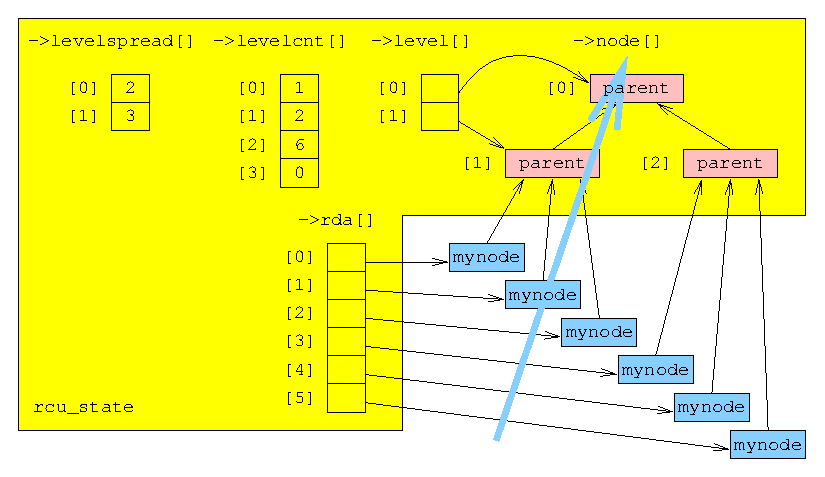
\includegraphics{appendix/rcuimpl/RCUTreeQSScan}}
\caption{Scanning {\tt rcu\_node} Structures When Applying Quiescent States}
\label{fig:app:rcuimpl:rcutree:Scanning rcu-node Structures When Applying Quiescent States}
\end{figure*}

Each pass through the loop spanning lines~6-23 does the required
processing for one level of the \co{rcu_node} hierarchy, traversing
the data structures as shown by the blue arrow in
Figure~\ref{fig:app:rcuimpl:rcutree:Scanning rcu-node Structures When Applying Quiescent States}.

Line~7 checks to see if all of the bits in \co{mask} have already
been cleared in the current \co{rcu_node} structure's \co{->qsmask}
field, and, if so, line~8 releases the lock and re-enables interrupts,
and line~9 returns to the caller.
If not, line~11 clears the bits specified by \co{mask} from the current
\co{rcu_node} structure's \co{qsmask} field.
Line~12 then checks to see if there are more bits remaining
in \co{->qsmask}, and, if so, line~13 releases the lock and re-enables
interrupts, and line~14 returns to the caller.

Otherwise, it is necessary to advance up to the next level of the
\co{rcu_node} hierarchy.
In preparation for this next level, line~16 places a mask with the
single bit set corresponding to the current \co{rcu_node} structure within
its parent.
Line~17 checks to see if there in fact is a parent for the current
\co{rcu_node} structure, and, if not, line~18 breaks from the
loop.
On the other hand, if there is a parent \co{rcu_node} structure,
line~20 releases the current \co{rcu_node} structure's lock,
line~21 advances the \co{rnp} local variable to the parent,
and line~22 acquires the parent's lock.
Execution then continues at the beginning of the loop on line~7.

If line~18 breaks from the loop, we know that the current grace period
has ended, as the only way that all bits can be cleared in the
root \co{rcu_node} structure is if all CPUs have passed through
quiescent states.
In this case, line~24 updates the \co{rcu_state} structure's
\co{->completed} field to match the number of the newly ended grace
period, indicating that the grace period has in fact ended.
Line~24 then invokes \co{rcu_process_gp_end()} to advance the
running CPU's RCU callbacks,
and, finally, line~26 invokes \co{rcu_start_gp()} in order to
start a new grace period should any remaining callbacks on the currently
running CPU require one.

\begin{figure}[tbp]
{ \scriptsize
\begin{verbatim}
  1 static void rcu_do_batch(struct rcu_data *rdp)
  2 {
  3   unsigned long flags;
  4   struct rcu_head *next, *list, **tail;
  5   int count;
  6
  7   if (!cpu_has_callbacks_ready_to_invoke(rdp))
  8     return;
  9   local_irq_save(flags);
 10   list = rdp->nxtlist;
 11   rdp->nxtlist = *rdp->nxttail[RCU_DONE_TAIL];
 12   *rdp->nxttail[RCU_DONE_TAIL] = NULL;
 13   tail = rdp->nxttail[RCU_DONE_TAIL];
 14   for (count = RCU_NEXT_SIZE - 1; count >= 0; count--)
 15     if (rdp->nxttail[count] ==
 16         rdp->nxttail[RCU_DONE_TAIL])
 17       rdp->nxttail[count] = &rdp->nxtlist;
 18   local_irq_restore(flags);
 19   count = 0;
 20   while (list) {
 21     next = list->next;
 22     prefetch(next);
 23     list->func(list);
 24     list = next;
 25     if (++count >= rdp->blimit)
 26       break;
 27   }
 28   local_irq_save(flags);
 29   rdp->qlen -= count;
 30   if (list != NULL) {
 31     *tail = rdp->nxtlist;
 32     rdp->nxtlist = list;
 33     for (count = 0; count < RCU_NEXT_SIZE; count++)
 34       if (&rdp->nxtlist == rdp->nxttail[count])
 35         rdp->nxttail[count] = tail;
 36       else
 37         break;
 38   }
 39   if (rdp->blimit == LONG_MAX && rdp->qlen <= qlowmark)
 40     rdp->blimit = blimit;
 41   local_irq_restore(flags);
 42   if (cpu_has_callbacks_ready_to_invoke(rdp))
 43     raise_softirq(RCU_SOFTIRQ);
 44 }
\end{verbatim}
}
\caption{Code for {\tt rcu\_do\_batch()}}
\label{fig:app:rcuimpl:rcutreewt:Code for rcu-do-batch}
\end{figure}

Figure~\ref{fig:app:rcuimpl:rcutreewt:Code for rcu-do-batch}
shows \co{rcu_do_batch()}, which invokes RCU callbacks
whose grace periods have ended.
Only callbacks on the running CPU will be invoked---other CPUs must
invoke their own callbacks.

\QuickQuiz{}
	How do RCU callbacks on dynticks-idle or offline CPUs
	get invoked?
\QuickQuizAnswer{
	They don't.
	CPUs with RCU callbacks are not permitted to enter dynticks-idle
	mode, so dynticks-idle CPUs never have RCU callbacks.
	When CPUs go offline, their RCU callbacks are migrated to
	an online CPU, so offline CPUs never have RCU callbacks, either.
	Thus, there is no need to invoke callbacks on dynticks-idle
	or offline CPUs.
} \QuickQuizEnd

Line~7 invokes \co{cpu_has_callbacks_ready_to_invoke()} to see if
this CPU has any RCU callbacks whose grace period has completed,
and, if not, line~8 returns.
Lines~9 and 18 disable and re-enable interrupts, respectively.
Lines~11-13 remove the ready-to-invoke callbacks from \co{->nxtlist},
and lines~14-17 make any needed adjustments to the tail pointers.

\QuickQuiz{}
	Why would lines~14-17 in
	Figure~\ref{fig:app:rcuimpl:rcutreewt:Code for rcu-do-batch}
	need to adjust the tail pointers?
\QuickQuizAnswer{
	If any of the tail pointers reference the last callback
	in the sublist that was ready to invoke, they must be
	changed to instead reference the \co{->nxtlist} pointer.
	This situation occurs when the sublists
	immediately following the ready-to-invoke sublist are empty.
} \QuickQuizEnd

Line~19 initializes local variable \co{count} to zero in preparation
for counting the number of callbacks that will actually be invoked.
Each pass through the loop spanning lines~20-27 invokes and counts
a callback, with lines~25-26 exiting the loop if too many callbacks
are to be invoked at a time (thus preserving responsiveness).
The remainder of the function then requeues any callbacks that could
not be invoked due to this limit.

Lines~28 and 41 disable and re-enable interrupts, respectively.
Line~29 updates the \co{->qlen} field, which maintains a count
of the total number of RCU callbacks for this CPU.
Line~30 checks to see if there were any ready-to-invoke callbacks
that could not be invoked at the moment due to the limit on the
number that may be invoked at a given time.
If such callbacks remain, lines~30-38 requeue them, again adjusting
the tail pointers as needed.
Lines~39-40 restore the batch limit if it was increased due to
excessive callback backlog, and lines~42-43 cause additional RCU
processing to be scheduled if there are any ready-to-invoke
callbacks remaining.

\subsection{Dyntick-Idle Functions}
\label{app:rcuimpl:rcutreewt:Dyntick-Idle Functions}

The functions in this section are defined only in \co{CONFIG_NO_HZ}
builds of the Linux kernel,
though in some cases, extended-no-op versions are present otherwise.
These functions control whether or not RCU pays attention to a given CPU.
CPUs in dynticks-idle mode are ignored, but only if they are not
currently in an interrupt or NMI handler.
The functions in this section communicate this CPU state to RCU.

This set of functions is greatly simplified from that used in
preemptible RCU, see
Section~\ref{sec:formal:Promela Parable: dynticks and Preemptible RCU}
for a description of the earlier more-complex model.
Manfred Spraul put forth the idea for this simplified interface in
one of his state-based RCU
patches~\cite{ManfredSpraul2008StateMachineRCU,ManfredSpraul2008dyntickIRQNMI}.

Section~\ref{app:rcuimpl:rcutreewt:Entering and Exiting Dyntick-Idle Mode}
describes the functions that enter and exit dynticks-idle mode from
process context,
Section~\ref{app:rcuimpl:rcutreewt:NMIs from Dyntick-Idle Mode}
describes the handling of NMIs from dynticks-idle mode,
Section~\ref{app:rcuimpl:rcutreewt:Interrupts from Dyntick-Idle Mode}
covers handling of interrupts from dynticks-idle mode, and
Section~\ref{app:rcuimpl:rcutreewt:Checking for Dyntick-Idle Mode}
presents functions that check whether some other CPU is currently in
dynticks-idle mode.

\subsubsection{Entering and Exiting Dyntick-Idle Mode}
\label{app:rcuimpl:rcutreewt:Entering and Exiting Dyntick-Idle Mode}

\begin{figure}[tbp]
{ \scriptsize
\begin{verbatim}
  1 void rcu_enter_nohz(void)
  2 {
  3   unsigned long flags;
  4   struct rcu_dynticks *rdtp;
  5
  6   smp_mb();
  7   local_irq_save(flags);
  8   rdtp = &__get_cpu_var(rcu_dynticks);
  9   rdtp->dynticks++;
 10   rdtp->dynticks_nesting--;
 11   local_irq_restore(flags);
 12 }
 13
 14 void rcu_exit_nohz(void)
 15 {
 16   unsigned long flags;
 17   struct rcu_dynticks *rdtp;
 18
 19   local_irq_save(flags);
 20   rdtp = &__get_cpu_var(rcu_dynticks);
 21   rdtp->dynticks++;
 22   rdtp->dynticks_nesting++;
 23   local_irq_restore(flags);
 24   smp_mb();
 25 }
\end{verbatim}
}
\caption{Entering and Exiting Dyntick-Idle Mode}
\label{fig:app:rcuimpl:rcutreewt:Entering and Exiting Dyntick-Idle Mode}
\end{figure}

Figure~\ref{fig:app:rcuimpl:rcutreewt:Entering and Exiting Dyntick-Idle Mode}
shows the \co{rcu_enter_nohz()} and \co{rcu_exit_nohz()} functions
that allow the scheduler to transition to and from dynticks-idle
mode.
Therefore, after \co{rcu_enter_nohz()} has been call, RCU will ignore
it, at least until the next \co{rcu_exit_nohz()}, the next interrupt,
or the next NMI.

Line~6 of \co{rcu_enter_nohz()} executes a memory barrier to ensure
that any preceding RCU read-side critical sections are seen to have
occurred before the following code that tells RCU to ignore this CPU.
Lines~7 and 11 disable and restore interrupts in order to avoid
interference with the state change.
Line~8 picks up a pointer to the running CPU's \co{rcu_dynticks}
structure, line~9 increments the \co{->dynticks} field (which now
must be even to indicate that this CPU may be ignored), and finally line~10
decrements the \co{->dynticks_nesting} field (which now must be
zero to indicate that there is no reason to pay attention to this CPU).

Lines~19 and 23 of \co{rcu_exit_nohz()} disable and re-enable interrupts,
again to avoid interference.
Line~20 obtains a pointer to this CPU's \co{rcu_dynticks} structure,
line~21 increments the \co{->dynticks} field (which now must be odd
in order to indicate that RCU must once again pay attention to this
CPU), and line~22 increments the \co{->dynticks_nesting} field
(which now must have the value 1 to indicate that there is one
reason to pay attention to this CPU).

\subsubsection{NMIs from Dyntick-Idle Mode}
\label{app:rcuimpl:rcutreewt:NMIs from Dyntick-Idle Mode}

\begin{figure}[tbp]
{ \scriptsize
\begin{verbatim}
  1 void rcu_nmi_enter(void)
  2 {
  3   struct rcu_dynticks *rdtp;
  4
  5   rdtp = &__get_cpu_var(rcu_dynticks);
  6   if (rdtp->dynticks & 0x1)
  7     return;
  8   rdtp->dynticks_nmi++;
  9   smp_mb();
 10 }
 11
 12 void rcu_nmi_exit(void)
 13 {
 14   struct rcu_dynticks *rdtp;
 15
 16   rdtp = &__get_cpu_var(rcu_dynticks);
 17   if (rdtp->dynticks & 0x1)
 18     return;
 19   smp_mb();
 20   rdtp->dynticks_nmi++;
\end{verbatim}
}
\caption{NMIs from Dyntick-Idle Mode}
\label{fig:app:rcuimpl:rcutreewt:NMIs from Dyntick-Idle Mode}
\end{figure}

Figure~\ref{fig:app:rcuimpl:rcutreewt:NMIs from Dyntick-Idle Mode}
shows \co{rcu_nmi_enter()} and \co{rcu_nmi_exit()}, which handle
NMI entry and exit, respectively.
It is important to keep in mind that entering an NMI handler
exits dyntick-idle mode and vice versa, in other words, RCU must
pay attention to CPUs that claim to be in dyntick-idle mode while
they are executing NMI handlers, due to the fact that NMI handlers
can contain RCU read-side critical sections.
This reversal of roles can be quite confusing: you have been warned.

Line~5 of \co{rcu_nmi_enter()} obtains a pointer to this CPU's
\co{rcu_dynticks} structure, and line~6 checks to see if this
CPU is already under scrutiny by RCU, with line~7 silently returning
if so.
Otherwise, line~8 increments the \co{->dynticks_nmi} field, which
must now have an odd-numbered value.
Finally, line~9 executes a memory barrier to ensure that the prior
increment of \co{->dynticks_nmi} is see by all CPUs to happen
before any subsequent RCU read-side critical section.

Line~16 of \co{rcu_nmi_exit()} again fetches a pointer to this CPU's
\co{rcu_dynticks} structure, and line~17 checks to see if RCU would
be paying attention to this CPU even if it were not in an NMI,
with line~18 silently returning if so.
Otherwise, line~19 executes a memory barrier to ensure that any
RCU read-side critical sections within the handler are seen by all
CPUs to happen before the increment of the \co{->dynticks_nmi} field
on line~20.
The new value of this field must now be even.

\QuickQuiz{}
	But how does the code in
	Figure~\ref{fig:app:rcuimpl:rcutreewt:NMIs from Dyntick-Idle Mode}
	handle nested NMIs?
\QuickQuizAnswer{
	It does not have to handle nested NMIs, because NMIs do not nest.
} \QuickQuizEnd

\subsubsection{Interrupts from Dyntick-Idle Mode}
\label{app:rcuimpl:rcutreewt:Interrupts from Dyntick-Idle Mode}

\begin{figure}[tbp]
{ \scriptsize
\begin{verbatim}
  1 void rcu_irq_enter(void)
  2 {
  3   struct rcu_dynticks *rdtp;
  4
  5   rdtp = &__get_cpu_var(rcu_dynticks);
  6   if (rdtp->dynticks_nesting++)
  7     return;
  8   rdtp->dynticks++;
  9   smp_mb();
 10 }
 11
 12 void rcu_irq_exit(void)
 13 {
 14   struct rcu_dynticks *rdtp;
 15
 16   rdtp = &__get_cpu_var(rcu_dynticks);
 17   if (--rdtp->dynticks_nesting)
 18     return;
 19   smp_mb();
 20   rdtp->dynticks++;
 21   if (__get_cpu_var(rcu_data).nxtlist ||
 22       __get_cpu_var(rcu_bh_data).nxtlist)
 23     set_need_resched();
 24 }
\end{verbatim}
}
\caption{Interrupts from Dyntick-Idle Mode}
\label{fig:app:rcuimpl:rcutreewt:Interrupts from Dyntick-Idle Mode}
\end{figure}

Figure~\ref{fig:app:rcuimpl:rcutreewt:Interrupts from Dyntick-Idle Mode}
shows \co{rcu_irq_enter()} and \co{rcu_irq_exit()}, which handle
interrupt entry and exit, respectively.
As with NMIs, it is important to note that entering an interrupt
handler exits dyntick-idle mode and vice versa, due to the fact
that RCU read-side critical sections can appear in interrupt handlers.

Line~5 of \co{rcu_irq_enter()} once again acquires a reference to
the current CPU's \co{rcu_dynticks} structure.
Line~6 increments the \co{->dynticks_nesting} field, and if the
original value was already non-zero (in other words, RCU was
already paying attention to this CPU), line~7 silently returns.
Otherwise, line~8 increments the  \co{->dynticks} field, which
then must have an odd-numbered value.
Finally, line~9 executes a memory barrier so that this increment
is seen by all CPUs as happening before any RCU read-side critical
sections that might be in the interrupt handler.

Line~16 of \co{rcu_irq_exit()} does the by-now traditional acquisition
of a reference to the currently running CPU's \co{rcu_dynticks} structure.
Line~17 decrements the \co{->dynticks_nesting} field, and, if the
result is non-zero (in other words, RCU must still pay attention
to this CPU despite exiting this interrupt handler), then line~18
silently returns.
Otherwise, line~19 executes a memory barrier so that any RCU read-side
critical sections that might have been in the interrupt handler are
seen by all CPUs as having happened before the increment on line~20
of the \co{->dynticks} field (which must now have an even-numbered
value).
Lines~21 and 22 check to see if the interrupt handler posted any
``rcu'' or ``rcu\_bh'' callbacks, and, if so, line~23 forces this
CPU to reschedule, which has the side-effect of forcing it out of
dynticks-idle mode, as is required to allow RCU to handle the
grace period required by these callbacks.

\subsubsection{Checking for Dyntick-Idle Mode}
\label{app:rcuimpl:rcutreewt:Checking for Dyntick-Idle Mode}

The \co{dyntick_save_progress_counter()} and
\co{rcu_implicit_dynticks_qs()} functions are used to check
whether a CPU is in dynticks-idle mode.
The \co{dyntick_save_progress_counter()} function is invoked first,
and returns non-zero if the CPU is currently in dynticks-idle mode.
If the CPU was not in dynticks-idle mode, for example, because it is
currently handling an interrupt or NMI, then the
\co{rcu_implicit_dynticks_qs()} function is called some jiffies later.
This function looks at the current state in conjunction with state
stored away by the earlier call to \co{dyntick_save_progress_counter()},
again returning non-zero if the CPU either is in dynticks-idle mode or
was in dynticks-idle mode during the intervening time.
The \co{rcu_implicit_dynticks_qs()} function may be invoked repeatedly,
if need be, until it returns true.

\begin{figure}[tbp]
{ \scriptsize
\begin{verbatim}
  1 static int
  2 dyntick_save_progress_counter(struct rcu_data *rdp)
  3 {
  4   int ret;
  5   int snap;
  6   int snap_nmi;
  7
  8   snap = rdp->dynticks->dynticks;
  9   snap_nmi = rdp->dynticks->dynticks_nmi;
 10   smp_mb();
 11   rdp->dynticks_snap = snap;
 12   rdp->dynticks_nmi_snap = snap_nmi;
 13   ret = ((snap & 0x1) == 0) && ((snap_nmi & 0x1) == 0);
 14   if (ret)
 15     rdp->dynticks_fqs++;
 16   return ret;
 17 }
\end{verbatim}
}
\caption{Code for {\tt dyntick\_\-save\_\-progress\_\-counter()}}
\label{fig:app:rcuimpl:rcutreewt:Code for dyntick-save-progress-counter}
\end{figure}

Figure~\ref{fig:app:rcuimpl:rcutreewt:Code for dyntick-save-progress-counter}
shows the code for \co{dyntick_save_progress_counter()}, which
is passed a given CPU-\co{rcu_state} pair's \co{rcu_data} structure.
Lines~8 and 9 take snapshots of the CPU's \co{rcu_dynticks} structure's
\co{->dynticks} and \co{->dynticks_nmi} fields,
and then line~10 executes a memory barrier to ensure that the snapshot
is seen by all CPUs to have happened before any later processing
depending on these values.
This memory barrier pairs up with those in \co{rcu_enter_nohz()},
\co{rcu_exit_nohz()}, \co{rcu_nmi_enter()}, \co{rcu_nmi_exit()},
\co{rcu_irq_enter()}, and \co{rcu_irq_exit()}.
Lines~11 and 12 store these two snapshots away so that they can be
accessed by a later call to \co{rcu_implicit_dynticks_qs()}.
Line~13 checks to see if both snapshots have even-numbered values,
indicating that the CPU in question was in neither non-idle process
state, an interrupt handler, nor an NMI handler.
If so, lines~14 and 15 increment the statistical counter
\co{->dynticks_fqs}, which is used only for tracing.
Either way, line~16 returns the indication of whether the CPU was
in dynticks-idle mode.

\QuickQuiz{}
	Why isn't there a memory barrier between lines~8 and 9 of
	Figure~\ref{fig:app:rcuimpl:rcutreewt:Code for dyntick-save-progress-counter}?
	Couldn't this cause the code to fetch even-numbered values
	from both the \co{->dynticks} and \co{->dynticks_nmi} fields,
	even though these two fields never were zero at the same time?
\QuickQuizAnswer{
	First, review the code in
	Figures~\ref{fig:app:rcuimpl:rcutreewt:Entering and Exiting Dyntick-Idle Mode},
	\ref{fig:app:rcuimpl:rcutreewt:NMIs from Dyntick-Idle Mode}, and
	\ref{fig:app:rcuimpl:rcutreewt:Interrupts from Dyntick-Idle Mode},
	and note that \co{dynticks} and \co{dynticks_nmi} will never
	have odd values simultaneously (see especially lines~6 and 17 of
	Figure~\ref{fig:app:rcuimpl:rcutreewt:NMIs from Dyntick-Idle Mode},
	and recall that interrupts cannot happen from NMIs).

	Of course, given the placement of the memory barriers in these
	functions, it might \emph{appear} to another CPU that both
	counters were odd at the same time, but logically this cannot
	happen, and would indicate that the CPU had in fact passed
	through dynticks-idle mode.

	Now, let's suppose that at the time line~8 fetches \co{->dynticks},
	the value of \co{->dynticks_nmi} was at odd number, and that at the
	time line~9 fetches \co{->dynticks_nmi}, the value of
	\co{->dynticks} was an odd number.
	Given that both counters cannot be odd simultaneously, there must
	have been a time between these two fetches when both counters
	were even, and thus a time when the CPU was in dynticks-idle
	mode, which is a quiescent state, as required.

	So, why can't the \co{&&} on line~13 of
	Figure~\ref{fig:app:rcuimpl:rcutreewt:Code for dyntick-save-progress-counter}
	be replaced with an \co{==}?
	Well, it could be, but this would likely be more confusing
	than helpful.
} \QuickQuizEnd

\begin{figure}[tbp]
{ \scriptsize
\begin{verbatim}
  1 static int
  2 rcu_implicit_dynticks_qs(struct rcu_data *rdp)
  3 {
  4   long curr;
  5   long curr_nmi;
  6   long snap;
  7   long snap_nmi;
  8
  9   curr = rdp->dynticks->dynticks;
 10   snap = rdp->dynticks_snap;
 11   curr_nmi = rdp->dynticks->dynticks_nmi;
 12   snap_nmi = rdp->dynticks_nmi_snap;
 13   smp_mb();
 14   if ((curr != snap || (curr & 0x1) == 0) &&
 15       (curr_nmi != snap_nmi || (curr_nmi & 0x1) == 0)) {
 16     rdp->dynticks_fqs++;
 17     return 1;
 18   }
 19   return rcu_implicit_offline_qs(rdp);
 20 }
\end{verbatim}
}
\caption{Code for {\tt rcu\_\-implicit\_\-dynticks\_\-qs()}}
\label{fig:app:rcuimpl:rcutreewt:Code for rcu-implicit-dynticks-qs}
\end{figure}

Figure~\ref{fig:app:rcuimpl:rcutreewt:Code for rcu-implicit-dynticks-qs}
shows the code for \co{rcu_implicit_dynticks_qs()}.
Lines~9-12 pick up both new values for the CPU's \co{rcu_dynticks}
structure's \co{->dynticks} and \co{->dynticks_nmi} fields, as well
as the snapshots taken by the last call to
\co{dyntick_save_progress_counter()}.
Line~13 then executes a memory barrier to ensure that the values are
seen by other CPUs to be gathered prior to subsequent RCU processing.
As with \co{dyntick_save_progress_counter()}, this memory barrier
pairs with those in \co{rcu_enter_nohz()},
\co{rcu_exit_nohz()}, \co{rcu_nmi_enter()}, \co{rcu_nmi_exit()},
\co{rcu_irq_enter()}, and \co{rcu_irq_exit()}.
Lines~14-15 then check to make sure that this CPU is either currently
in dynticks-idle mode (\co{(curr & 0x1) == 0} and
\co{(curr_nmi & 0x1) == 0}) or has passed through dynticks-idle mode
since the last call to \co{dyntick_save_progress_counter()}
(\co{curr != snap} and \co{curr_nmi != snap_nmi}).
If so, line~16 increments the \co{->dynticks_fqs} statistical
counter (again, used only for tracing) and line~17 returns non-zero
to indicate that the specified CPU has passed through a quiescent state.
Otherwise, line~19 invokes \co{rcu_implicit_offline_qs()}
(described in Section~\ref{app:rcuimpl:rcutreewt:Forcing Quiescent States})
to check whether the specified CPU is currently offline.

\subsection{Forcing Quiescent States}
\label{app:rcuimpl:rcutreewt:Forcing Quiescent States}

Normally, CPUs pass through quiescent states which are duly recorded,
so that grace periods end in a timely manner.
However, any of the following three conditions can prevent CPUs from
passing through quiescent states:

\begin{enumerate}
\item	The CPU is in dyntick-idle state, and is sleeping in a low-power
	mode.
	Although such a CPU is officially in an extended quiescent state,
	because it is not executing instructions, it cannot do anything
	on its own.
\item	The CPU is in the process of coming online, and RCU has been
	informed that it is online, but this CPU is not yet actually
	executing code, nor is it marked as online in \co{cpu_online_map}.
	The current grace period will therefore wait on it, but it cannot
	yet pass through quiescent states on its own.
\item	The CPU is running user-level code, but has avoided
	entering the scheduler for an extended time period.
\end{enumerate}

In each of these cases, RCU needs to take action on behalf of the
non-responding CPU.
The following sections describe the functions that take such action.
Section~\ref{app:rcuimpl:rcutreewt:Recording and Recalling Dynticks-Idle Grace Period}
describes the functions that record and recall the dynticks-idle
grace-period number (in order to avoid incorrectly applying a dynticks-idle
quiescent state to the wrong grace period),
Section~\ref{app:rcuimpl:rcutreewt:Handling Offline and Holdout CPUs}
describes functions that detect offline and holdout CPUs,
Section~\ref{app:rcuimpl:rcutreewt:Scanning for Holdout CPUs}
covers \co{rcu_process_dyntick()}, which scans for holdout CPUs, and
Section~\ref{app:rcuimpl:rcutreewt:Code for force-quiescent-state}
describes \co{force_quiescent_state()}, which drives the process of
detecting extended quiescent states and forcing quiescent states on
holdout CPUs.

\subsubsection{Recording and Recalling Dynticks-Idle Grace Period}
\label{app:rcuimpl:rcutreewt:Recording and Recalling Dynticks-Idle Grace Period}

\begin{figure}[tbp]
{ \scriptsize
\begin{verbatim}
  1 static void
  2 dyntick_record_completed(struct rcu_state *rsp,
  3                          long comp)
  4 {
  5   rsp->dynticks_completed = comp;
  6 }
  7
  8 static long
  9 dyntick_recall_completed(struct rcu_state *rsp)
 10 {
 11   return rsp->dynticks_completed;
 12 }
\end{verbatim}
}
\caption{Recording and Recalling Dynticks-Idle Grace Period}
\label{fig:app:rcuimpl:rcutreewt:Recording and Recalling Dynticks-Idle Grace Period}
\end{figure}

Figure~\ref{fig:app:rcuimpl:rcutreewt:Recording and Recalling Dynticks-Idle Grace Period}
shows the code for \co{dyntick_record_completed()} and
\co{dyntick_recall_completed()}.
These functions are defined as shown only if dynticks
is enabled (in other words, the \co{CONFIG_NO_HZ} kernel parameter
is selected), otherwise they are essentially no-ops.
The purpose of these functions is to ensure that a given observation
of a CPU in dynticks-idle mode is associated with the correct
grace period in face of races between reporting this CPU in
dynticks-idle mode and this CPU coming out of dynticks-idle mode
and reporting a quiescent state on its own.

Lines~1-6 show \co{dyntick_record_completed()}, which stores the
value specified by its \co{comp} argument into the specified
\co{rcu_state} structure's \co{->dynticks_completed} field.
Lines~8-12 show \co{dyntick_recall_completed()}, which returns
the value stored by the most recent call to
\co{dyntick_record_completed()} for this combination of CPU and
\co{rcu_state} structure.

\subsubsection{Handling Offline and Holdout CPUs}
\label{app:rcuimpl:rcutreewt:Handling Offline and Holdout CPUs}

\begin{figure}[tbp]
{ \scriptsize
\begin{verbatim}
  1 static int rcu_implicit_offline_qs(struct rcu_data *rdp)
  2 {
  3   if (cpu_is_offline(rdp->cpu)) {
  4     rdp->offline_fqs++;
  5     return 1;
  6   }
  7   if (rdp->cpu != smp_processor_id())
  8     smp_send_reschedule(rdp->cpu);
  9   else
 10     set_need_resched();
 11   rdp->resched_ipi++;
 12   return 0;
 13 }
\end{verbatim}
}
\caption{Handling Offline and Holdout CPUs}
\label{fig:app:rcuimpl:rcutreewt:Handling Offline and Holdout CPUs}
\end{figure}

Figure~\ref{fig:app:rcuimpl:rcutreewt:Handling Offline and Holdout CPUs}
shows the code for \co{rcu_implicit_offline_qs()}, which checks for
offline CPUs and forcing online holdout CPUs to enter a quiescent state.

Line~3 checks to see if the specified CPU is offline, and, if so,
line~4 increments statistical counter \co{->offline_fqs} (which is
used only for tracing), and line~5 returns non-zero to indicate
that the CPU is in an extended quiescent state.

Otherwise, the CPU is online, not in dynticks-idle mode (or this
function would not have been called in the first place), and has
not yet passed through a quiescent state for this grace period.
Line~7 checks to see if the holdout CPU is the current running
CPU, and, if not, line~8 sends the holdout CPU a reschedule IPI.
Otherwise, line~10 sets the \co{TIF_NEED_RESCHED} flag for the
current task, forcing the current CPU into the scheduler.
In either case, the CPU should then quickly enter a quiescent
state.
Line~11 increments statistical counter \co{resched_ipi}, which is
again used only for tracing.
Finally, line~12 returns zero to indicate that the holdout CPU is
still refusing to pass through a quiescent state.

\subsubsection{Scanning for Holdout CPUs}
\label{app:rcuimpl:rcutreewt:Scanning for Holdout CPUs}

\begin{figure}[tbp]
{ \scriptsize
\begin{verbatim}
  1 static int
  2 rcu_process_dyntick(struct rcu_state *rsp,
  3                     long lastcomp,
  4                     int (*f)(struct rcu_data *))
  5 {
  6   unsigned long bit;
  7   int cpu;
  8   unsigned long flags;
  9   unsigned long mask;
 10   struct rcu_node *rnp_cur;
 11   struct rcu_node *rnp_end;
 12
 13   rnp_cur = rsp->level[NUM_RCU_LVLS - 1];
 14   rnp_end = &rsp->node[NUM_RCU_NODES];
 15   for (; rnp_cur < rnp_end; rnp_cur++) {
 16     mask = 0;
 17     spin_lock_irqsave(&rnp_cur->lock, flags);
 18     if (rsp->completed != lastcomp) {
 19       spin_unlock_irqrestore(&rnp_cur->lock, flags);
 20       return 1;
 21     }
 22     if (rnp_cur->qsmask == 0) {
 23       spin_unlock_irqrestore(&rnp_cur->lock, flags);
 24       continue;
 25     }
 26     cpu = rnp_cur->grplo;
 27     bit = 1;
 28     for (; cpu <= rnp_cur->grphi; cpu++, bit <<= 1) {
 29       if ((rnp_cur->qsmask & bit) != 0 &&
 30           f(rsp->rda[cpu]))
 31         mask |= bit;
 32     }
 33     if (mask != 0 && rsp->completed == lastcomp) {
 34       cpu_quiet_msk(mask, rsp, rnp_cur, flags);
 35       continue;
 36     }
 37     spin_unlock_irqrestore(&rnp_cur->lock, flags);
 38   }
 39   return 0;
 40 }
\end{verbatim}
}
\caption{Scanning for Holdout CPUs}
\label{fig:app:rcuimpl:rcutreewt:Scanning for Holdout CPUs}
\end{figure}

\begin{figure*}[tb]
\centering
\resizebox{6in}{!}{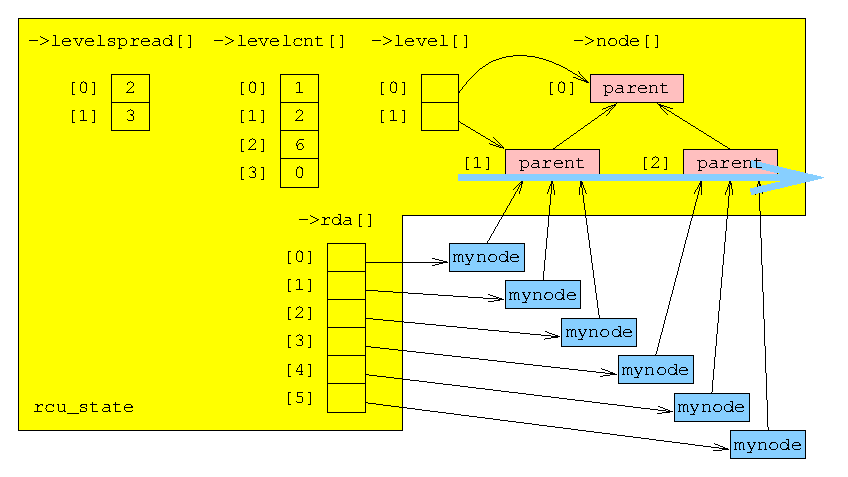
\includegraphics{appendix/rcuimpl/RCUTreeLeafScan}}
\caption{Scanning Leaf {\tt rcu\_node} Structures}
\label{fig:app:rcuimpl:rcutree:Scanning Leaf rcu-node Structures}
\end{figure*}

Figure~\ref{fig:app:rcuimpl:rcutreewt:Scanning for Holdout CPUs}
shows the code for \co{rcu_process_dyntick()}, which scans the
leaf \co{rcu_node} structures in search of holdout CPUs,
as illustrated by the blue arrow in
Figure~\ref{fig:app:rcuimpl:rcutree:Scanning Leaf rcu-node Structures}.
It invokes the function passed in through argument \co{f} on each
such CPU's \co{rcu_data} structure, and returns non-zero if
the grace period specified by the \co{lastcomp} argument has ended.

Lines~13 and 14 acquire references to the first and the last leaf
\co{rcu_node} structures, respectively.
Each pass through the loop spanning lines~15-38 processes one of
the leaf \co{rcu_node} structures.

Line~16 sets the local variable \co{mask} to zero.
This variable will be used to accumulate the CPUs within the current
leaf \co{rcu_node} structure that are in extended quiescent states, and
can thus be reported as such.
Line~17 acquires the current leaf \co{rcu_node} structure's lock,
and line~18 checks to see if the current grace period has completed,
and, if so, line~19 releases the lock and line~20 returns non-zero.
Otherwise, line~22 checks for holdout CPUs associated with this
\co{rcu_node} structure, and, if there are none, line~23 releases
the lock and line~24 restarts the loop from the beginning on the
next leaf \co{rcu_node} structure.

Execution reaches line~26 if there is at least one holdout CPU associated
with this \co{rcu_node} structure.
Lines~26 and 27 set local variables \co{cpu} and \co{bit} to reference
the lowest-numbered CPU associated with this \co{rcu_node} structure.
Each pass through the loop spanning lines~28-32 checks one of the
CPUs associated with the current \co{rcu_node} structure.
Line~29 checks to see if the this CPU is still holding out or if
it has already passed through a quiescent state.
If it is still a holdout, line~30 invokes the specified function
(either \co{dyntick_save_progress_counter()} or
\co{rcu_implicit_dynticks_qs()}, as specified by the caller), and
if that function returns non-zero (indicating that the current CPU
is in an extended quiescent state), then line~31 sets the current
CPU's bit in \co{mask}.

Line 33 then checks to see if any CPUs were identified as being
in extended quiescent states and if the current grace period is
still in force, and, if so, line~34 invokes \co{cpu_quiet_msk()}
to report that the grace period need no longer wait for those
CPUs and then line~35 restarts the loop with the next \co{rcu_node}
structure.
(Note that \co{cpu_quiet_msk()} releases the current \co{rcu_node}
structure's lock, and might well end the current grace period.)
Otherwise, if all holdout CPUs really are still holding out, line~37
releases the current \co{rcu_node} structure's lock.

Once all of the leaf \co{rcu_node} structures have been processed,
the loop exits, and line~39 returns zero to indicate that the current
grace period is still in full force.
(Recall that line~20 returns non-zero should the current grace period
come to an end.)

\subsubsection{Code for {\tt force\_quiescent\_state()}}
\label{app:rcuimpl:rcutreewt:Code for force-quiescent-state}

\begin{figure}[tbp]
{ \scriptsize
\begin{verbatim}
  1 static void
  2 force_quiescent_state(struct rcu_state *rsp, int relaxed)
  3 {
  4   unsigned long flags;
  5   long lastcomp;
  6   struct rcu_data *rdp = rsp->rda[smp_processor_id()];
  7   struct rcu_node *rnp = rcu_get_root(rsp);
  8   u8 signaled;
  9
 10   if (ACCESS_ONCE(rsp->completed) ==
 11       ACCESS_ONCE(rsp->gpnum))
 12     return;
 13   if (!spin_trylock_irqsave(&rsp->fqslock, flags)) {
 14     rsp->n_force_qs_lh++;
 15     return;
 16   }
 17   if (relaxed &&
 18       (long)(rsp->jiffies_force_qs - jiffies) >= 0 &&
 19       (rdp->n_rcu_pending_force_qs -
 20        rdp->n_rcu_pending) >= 0)
 21     goto unlock_ret;
 22   rsp->n_force_qs++;
 23   spin_lock(&rnp->lock);
 24   lastcomp = rsp->completed;
 25   signaled = rsp->signaled;
 26   rsp->jiffies_force_qs =
 27     jiffies + RCU_JIFFIES_TILL_FORCE_QS;
 28   rdp->n_rcu_pending_force_qs =
 29     rdp->n_rcu_pending +
 30     RCU_JIFFIES_TILL_FORCE_QS;
 31   if (lastcomp == rsp->gpnum) {
 32     rsp->n_force_qs_ngp++;
 33     spin_unlock(&rnp->lock);
 34     goto unlock_ret;
 35   }
 36   spin_unlock(&rnp->lock);
 37   switch (signaled) {
 38   case RCU_GP_INIT:
 39     break;
 40   case RCU_SAVE_DYNTICK:
 41     if (RCU_SIGNAL_INIT != RCU_SAVE_DYNTICK)
 42       break;
 43     if (rcu_process_dyntick(rsp, lastcomp,
 44           dyntick_save_progress_counter))
 45       goto unlock_ret;
 46     spin_lock(&rnp->lock);
 47     if (lastcomp == rsp->completed) {
 48       rsp->signaled = RCU_FORCE_QS;
 49       dyntick_record_completed(rsp, lastcomp);
 50     }
 51     spin_unlock(&rnp->lock);
 52     break;
 53   case RCU_FORCE_QS:
 54     if (rcu_process_dyntick(rsp,
 55           dyntick_recall_completed(rsp),
 56           rcu_implicit_dynticks_qs))
 57       goto unlock_ret;
 58     break;
 59   }
 60 unlock_ret:
 61   spin_unlock_irqrestore(&rsp->fqslock, flags);
 62 }
\end{verbatim}
}
\caption{{\tt force\_quiescent\_state()} Code}
\label{fig:app:rcuimpl:rcutreewt:Code for rcutree force-quiescent-state}
\end{figure}

Figure~\ref{fig:app:rcuimpl:rcutreewt:Code for rcutree force-quiescent-state}
shows the code for \co{force_quiescent_state()} for
\co{CONFIG_SMP},\footnote{
	For non-\co{CONFIG_SMP}, \co{force_quiescent_state} is a
	simple wrapper around \co{set_need_resched()}.}
which is invoked when RCU feels the need to expedite the current
grace period by forcing CPUs through quiescent states.
RCU feels this need when either:
\begin{enumerate}
\item	the current grace period has gone on for more than three jiffies
	(or as specified by the compile-time value of
	\co{RCU_JIFFIES_TILL_FORCE_QS}), or
\item	a CPU enqueuing an RCU callback via either \co{call_rcu()}
	or \co{call_rcu_bh()} sees more than 10,000 callbacks enqueued
	(or as specified by the boot-time parameter \co{qhimark}).
\end{enumerate}

Lines~10-12 check to see if there is a grace period in progress,
silently exiting if not.
Lines~13-16 attempt to acquire \co{->fqslock}, which prevents concurrent
attempts to expedite a grace period.
The \co{->n_force_qs_lh} counter is incremented when this lock is
already held, and is visible via the \co{fqlh=} field
in the \co{rcuhier} debugfs file when the \co{CONFIG_RCU_TRACE} kernel
parameter is enabled.
Lines~17-21 check to see if it is really necessary to expedite the
current grace period, in other words, if (1) the current CPU has 10,000
RCU callbacks waiting, or (2) at least three jiffies have passed
since either the beginning of the current grace period or since the
last attempt to expedite the current grace period, measured either
by the \co{jiffies} counter or by the number of calls to
\co{rcu_pending}.
Line~22 then counts the number of attempts to expedite grace periods.

Lines~23-36 are executed with the root \co{rcu_node} structure's lock
held in order to prevent confusion should the current grace period
happen to end just as we try to expedite it.
Lines~24 and 25 snapshot the \co{->completed} and \co{->signaled} fields,
lines~26-30 set the soonest time that a subsequent non-relaxed
\co{force_quiescent_state()} will be allowed to actually do
any expediting, and lines~31-35 check to see if the grace period
ended while we were acquiring the \co{rcu_node} structure's lock,
releasing this lock and returning if so.

Lines~37-59 drive the \co{force_quiescent_state()} state machine.
If the grace period is still in the midst of initialization,
lines~41 and 42 simply return, allowing \co{force_quiescent_state()}
to be called again at a later time, presumably after initialization
has completed.
If dynticks are enabled (via the \co{CONFIG_NO_HZ} kernel
parameter), the first post-initialization call
to \co{force_quiescent_state()} in a given grace period will
execute lines~40-52, and the second and subsequent calls will
execute lines~53-59.
On the other hand, if dynticks is not enabled, then all post-initialization
calls to \co{force_quiescent_state()} will execute lines~53-59.

The purpose of lines~40-52 is to record the current dynticks-idle state
of all CPUs that have not yet passed through a quiescent state, and
to record a quiescent state for any that are currently in dynticks-idle
state (but not currently in an irq or NMI handler).
Lines~41-42 serve to inform gcc that this branch of the switch statement
is dead code for non-\co{CONFIG_NO_HZ} kernels.
Lines 43-45 invoke \co{rcu_process_dyntick()} in order to invoke
\co{dyntick_save_progress_counter()} for each CPU that has not yet
passed through a quiescent state for the current grace period,
exiting \co{force_quiescent_state()} if the grace period ends in
the meantime (possibly due to having found that all the CPUs that
had not yet passed through a quiescent state were sleeping in
dyntick-idle mode).
Lines~46 and 51 acquire and release the root \co{rcu_node} structure's
lock, again to avoid possible confusion with a concurrent end of the
current grace period.
Line~47 checks to see if the current grace period is still in force, and,
if so, line~48 advances the state machine to the \co{RCU_FORCE_QS} state
and line~49 saves the current grace-period number for the benefit of
the next invocation of \co{force_quiescent_state()}.
The reason for saving the current grace-period number is to correctly
handle race conditions involving the current grace period ending
concurrently with the next invocation of \co{force_quiescent_state()}.

As noted earlier, lines~53-58 handle the second and subsequent invocations
of \co{force_quiescent_state()} in \co{CONFIG_NO_HZ} kernels, and \emph{all}
invocations in non-\co{CONFIG_NO_HZ} kernels.
Lines~54 and 58 invoke \co{rcu_process_dyntick()}, which cycles through
the CPUs that have still not passed through a quiescent state, invoking
\co{rcu_implicit_dynticks_qs()} on them, which in turn checks to see
if any of these CPUs have passed through dyntick-idle state (if
\co{CONFIG_NO_HZ} is enabled), checks to see if we are waiting on
any offline CPUs, and finally sends a reschedule IPI to any remaining
CPUs not in the first two groups.

\subsection{CPU-Stall Detection}
\label{app:rcuimpl:rcutreewt:CPU-Stall Detection}

RCU checks for stalled CPUs when the \co{CONFIG_RCU_CPU_STALL_DETECTOR}
kernel parameter is selected.
``Stalled CPUs'' are those spinning in the kernel with preemption disabled,
which degrades response time.
These checks are implemented via the \co{record_gp_stall_check_time()},
\co{check_cpu_stall()}, \co{print_cpu_stall()}, and
\co{print_other_cpu_stall()} functions, each of which is described
below.
All of these functions are no-ops when the \co{CONFIG_RCU_CPU_STALL_DETECTOR}
kernel parameter is not selected.

\begin{figure}[tbp]
{ \scriptsize
\begin{verbatim}
  1 static void
  2 record_gp_stall_check_time(struct rcu_state *rsp)
  3 {
  4   rsp->gp_start = jiffies;
  5   rsp->jiffies_stall =
  6       jiffies + RCU_SECONDS_TILL_STALL_CHECK;
  7 }
\end{verbatim}
}
\caption{{\tt record\_gp\_stall\_check\_time()} Code}
\label{fig:app:rcuimpl:rcutreewt:Code for record-gp-stall-check-time}
\end{figure}

Figure~\ref{fig:app:rcuimpl:rcutreewt:Code for record-gp-stall-check-time}
shows the code for \co{record_gp_stall_check_time()}.
Line~4 records the current time (of the start of the grace period)
in jiffies, and lines~5-6 record the time at which CPU stalls should
be checked for, should the grace period run on that long.

\begin{figure}[tbp]
{ \scriptsize
\begin{verbatim}
  1 static void
  2 check_cpu_stall(struct rcu_state *rsp,
  3                 struct rcu_data *rdp)
  4 {
  5   long delta;
  6   struct rcu_node *rnp;
  7
  8   delta = jiffies - rsp->jiffies_stall;
  9   rnp = rdp->mynode;
 10   if ((rnp->qsmask & rdp->grpmask) && delta >= 0) {
 11     print_cpu_stall(rsp);
 12   } else if (rsp->gpnum != rsp->completed &&
 13        delta >= RCU_STALL_RAT_DELAY) {
 14     print_other_cpu_stall(rsp);
 15   }
 16 }
\end{verbatim}
}
\caption{{\tt check\_cpu\_stall()} Code}
\label{fig:app:rcuimpl:rcutreewt:Code for check-cpu-stall}
\end{figure}

Figure~\ref{fig:app:rcuimpl:rcutreewt:Code for check-cpu-stall}
shows the code for \co{check_cpu_stall}, which checks to see
if the grace period has stretched on too long, invoking either
\co{print_cpu_stall()} or \co{print_other_cpu_stall()} in order
to print a CPU-stall warning message if so.

Line~8 computes the number of jiffies since the time at which stall
warnings should be printed, which will be negative if it is not
yet time to print warnings.
Line~9 obtains a pointer to the leaf \co{rcu_node}
structure corresponding to the current CPU,
and line~10 checks to see if the current CPU has not yet passed through
a quiescent state and if the grace period has extended too long
(in other words, if the current CPU is stalled),
with line~11 invoking \co{print_cpu_stall()} if so.

Otherwise, lines~12-13 check to see if the grace period is still in effect
and if it has extended a couple of jiffies past the CPU-stall warning
duration, with line~14 invoking \co{print_other_cpu_stall()} if so.

\QuickQuiz{}
	Why wait the extra couple jiffies on lines~12-13 in
	Figure~\ref{fig:app:rcuimpl:rcutreewt:Code for check-cpu-stall}?
\QuickQuizAnswer{
	This added delay gives the offending CPU a better chance of
	reporting on itself, thus getting a decent stack trace of
	the stalled code.
	Of course, if the offending CPU is spinning with interrupts
	disabled, it will never report on itself, so other CPUs
	do so after a short delay.
} \QuickQuizEnd

\begin{figure}[tbp]
{ \scriptsize
\begin{verbatim}
  1 static void print_cpu_stall(struct rcu_state *rsp)
  2 {
  3   unsigned long flags;
  4   struct rcu_node *rnp = rcu_get_root(rsp);
  5
  6   printk(KERN_ERR
  7          "INFO: RCU detected CPU %d stall "
  8          "(t=%lu jiffies)\n",
  9     smp_processor_id(),
 10     jiffies - rsp->gp_start);
 11   dump_stack();
 12   spin_lock_irqsave(&rnp->lock, flags);
 13   if ((long)(jiffies - rsp->jiffies_stall) >= 0)
 14     rsp->jiffies_stall =
 15       jiffies + RCU_SECONDS_TILL_STALL_RECHECK;
 16   spin_unlock_irqrestore(&rnp->lock, flags);
 17   set_need_resched();
 18 }
\end{verbatim}
}
\caption{{\tt print\_cpu\_stall()} Code}
\label{fig:app:rcuimpl:rcutreewt:Code for print-cpu-stall}
\end{figure}

Figure~\ref{fig:app:rcuimpl:rcutreewt:Code for print-cpu-stall}
shows the code for \co{print_cpu_stall()}.

Line~6-11 prints a console message and dumps the current CPU's stack,
while lines~12-17 compute the time to the next CPU stall warning, should
the grace period stretch on that much additional time.

\QuickQuiz{}
	What prevents the grace period from ending before the
	stall warning is printed in
	Figure~\ref{fig:app:rcuimpl:rcutreewt:Code for print-cpu-stall}?
\QuickQuizAnswer{
	The caller checked that this CPU still had not reported a
	quiescent state, and because preemption is disabled, there is
	no way that a quiescent state could have been reported in
	the meantime.
} \QuickQuizEnd

\begin{figure}[tbp]
{ \scriptsize
\begin{verbatim}
  1 static void print_other_cpu_stall(struct rcu_state *rsp)
  2 {
  3   int cpu;
  4   long delta;
  5   unsigned long flags;
  6   struct rcu_node *rnp = rcu_get_root(rsp);
  7   struct rcu_node *rnp_cur;
  8   struct rcu_node *rnp_end;
  9
 10   rnp_cur = rsp->level[NUM_RCU_LVLS - 1];
 11   rnp_end = &rsp->node[NUM_RCU_NODES];
 12   spin_lock_irqsave(&rnp->lock, flags);
 13   delta = jiffies - rsp->jiffies_stall;
 14   if (delta < RCU_STALL_RAT_DELAY ||
 15       rsp->gpnum == rsp->completed) {
 16     spin_unlock_irqrestore(&rnp->lock, flags);
 17     return;
 18   }
 19   rsp->jiffies_stall = jiffies +
 20       RCU_SECONDS_TILL_STALL_RECHECK;
 21   spin_unlock_irqrestore(&rnp->lock, flags);
 22   printk(KERN_ERR "INFO: RCU detected CPU stalls:");
 23   for (; rnp_cur < rnp_end; rnp_cur++) {
 24     if (rnp_cur->qsmask == 0)
 25       continue;
 26     cpu = 0;
 27     for (; cpu <= rnp_cur->grphi - rnp_cur->grplo; cpu++)
 28       if (rnp_cur->qsmask & (1UL << cpu))
 29         printk(" %d", rnp_cur->grplo + cpu);
 30   }
 31   printk(" (detected by %d, t=%ld jiffies)\n",
 32          smp_processor_id(),
 33          (long)(jiffies - rsp->gp_start));
 34   force_quiescent_state(rsp, 0);
 35 }
\end{verbatim}
}
\caption{{\tt print\_other\_cpu\_stall()} Code}
\label{fig:app:rcuimpl:rcutreewt:Code for print-other-cpu-stall}
\end{figure}

Figure~\ref{fig:app:rcuimpl:rcutreewt:Code for print-other-cpu-stall}
shows the code for \co{print_other_cpu_stall()}, which prints out
stall warnings for CPUs other than the currently running CPU.

Lines~10 and 11 pick up references to the first leaf \co{rcu_node}
structure and one past the last leaf \co{rcu_node} structure,
respectively.
Line~12 acquires the root \co{rcu_node} structure's lock, and also
disables interrupts.
Line~13 calculates the how long ago the CPU-stall warning time occurred
(which will be negative if it has not yet occurred), and lines~14 and 15
check to see if the CPU-stall warning time has passed and if the
grace period has not yet ended,
with line~16 releasing the lock (and re-enabling interrupts) and
line~17 returning if so.

\QuickQuiz{}
	Why does \co{print_other_cpu_stall()} in
	Figure~\ref{fig:app:rcuimpl:rcutreewt:Code for print-other-cpu-stall}
	need to check for the grace period ending when
	\co{print_cpu_stall()} did not?
\QuickQuizAnswer{
	The other CPUs might pass through a quiescent state at any time,
	so the grace period might well have ended in the meantime.
} \QuickQuizEnd

Otherwise, lines~19 and 20 compute the next time that CPU stall warnings
should be printed (if the grace period extends that long) and
line~21 releases the lock and re-enables interrupts.
Lines~23-33 print a list of the stalled CPUs, and, finally,
line~34 invokes \co{force_quiescent_state()} in order to nudge the
offending CPUs into passing through a quiescent state.

\subsection{Possible Flaws and Changes}
\label{app:rcuimpl:rcutreewt:Possible Flaws and Changes}

The biggest possible issue with Hierarchical RCU put forward as of this
writing is the fact that \co{force_quiescent_state()} involves a
potential walk through all CPUs' \co{rcu_data} structures.
On a machine with thousands of CPUs, this could potentially represent
an excessive impact on scheduling latency, given that this scan is
conducted with interrupts disabled.

Should this become a problem in real life, one fix is to maintain
separate \co{force_quiescent_state()} sequencing on a
per-leaf-\co{rcu_node} basis as well as the current per-\co{rcu_state}
\co{->signaled} state variable.
This would allow incremental forcing of quiescent states on a
per-leaf-\co{rcu_node} basis, greatly reducing the worst-case degradation
of scheduling latency.

In the meantime, those caring deeply about scheduling latency can
limit the number of CPUs in the system or use the preemptible RCU
implementation.
